\documentclass[11pt]{article}
\usepackage[T1]{fontenc}
\usepackage{lmodern}
\usepackage[margin=1.05in]{geometry}
\usepackage{amsmath,amssymb,amsthm,mathtools}
\usepackage{microtype}
\usepackage{enumitem}
\usepackage{float}
\usepackage{booktabs,array}
\usepackage{tikz}
\usetikzlibrary{arrows.meta,calc,patterns,positioning,decorations.pathreplacing}
\usepackage{xcolor}
\definecolor{linkblue}{RGB}{25,55,100}
\usepackage[colorlinks=true,linkcolor=linkblue,citecolor=linkblue,urlcolor=linkblue]{hyperref}
\hypersetup{pdftitle={A Torsion-Free Group Algebra That Is Not Directly Finite},pdfauthor={OpenAI}}
\numberwithin{equation}{section}
\newtheorem{theorem}{Theorem}[section]
\newtheorem{proposition}[theorem]{Proposition}
\newtheorem{lemma}[theorem]{Lemma}
\newtheorem{corollary}[theorem]{Corollary}
\theoremstyle{definition}
\newtheorem{definition}[theorem]{Definition}
\theoremstyle{remark}
\newtheorem{remark}[theorem]{Remark}
\newcommand{\Ftwo}{\mathbb F_2}
\newcommand{\companionid}[1]{\begingroup\ttfamily\hyphenchar\font=`\-\relax #1\endgroup}
\DeclareMathOperator{\dist}{dist}
\DeclareMathOperator{\diam}{diam}
\DeclareMathOperator{\supp}{supp}
\title{A Torsion-Free Group Algebra That Is Not Directly Finite}
\author{OpenAI}
\date{October 4, 2026}

\begin{document}
\maketitle
\begin{abstract}
We construct a finitely presented torsion-free counterexample to Kaplansky's
direct finiteness conjecture over the field of two elements. The group admits
a finite two-dimensional classifying complex.
\end{abstract}

\section{Introduction}\label{sec:introduction}

A unital ring $R$ is \emph{directly finite} if $ab=1$ implies $ba=1$ for all
$a,b\in R$. For a field $K$ and a group $G$, the group algebra $K[G]$ consists
of finite formal sums of elements of $G$ with coefficients in $K$, with
multiplication extending the group operation bilinearly. Kaplansky's direct
finiteness conjecture asserts that every such group algebra is directly finite.
We prove that the implication can fail even when the field is finite and the
group is finitely presented and torsion-free.
A classifying complex for $G$ is a connected CW complex with fundamental group
$G$ and contractible universal cover.

\begin{theorem}\label{thm:main}
There exist a finitely presented torsion-free group $G$ and elements
$a,b,c\in\Ftwo[G]$ such that
\[
 ab=1,\qquad ac=0,\qquad c\ne0.
\]
Consequently $ba\ne1$. The group $G$ admits a finite two-dimensional
classifying complex.
\end{theorem}

The auxiliary element $c$ certifies failure of the reverse identity:
if $ba=1$, then $c=(ba)c=b(ac)=0$.

\subsection*{History and related work}
Kaplansky's formulation separates the characteristic-zero theorem from the
positive-characteristic question~\cite[Part~II, Section~3, Problem~2,
pp.~122--123]{Kaplansky1972}. In characteristic zero, group algebras are directly
finite for every group. The operator-algebra argument also applies to matrix
rings; Montgomery gave a concise $C^*$-algebra proof~\cite{Montgomery1969}.
A ring whose matrix rings of every finite size are directly finite is called
\emph{stably finite}.

In arbitrary characteristic, Ara, O'Meara, and Perera proved stable finiteness
for group algebras of free-by-amenable groups over division
rings~\cite{AraOMearaPerera2002}. Elek and Szab\'o extended the conclusion to
sofic groups~\cite[Corollary~4.7]{ElekSzabo2004}, a class defined by finite
approximate permutation actions. Their theorem implies that the group in
Theorem~\ref{thm:main} is not sofic. A complementary approach studies the
finite cancellation patterns forced by a one-sided inverse. Dykema, Heister,
and Juschenko organized these patterns into universal groups and established
direct finiteness for several small support pairs over
$\Ftwo$~\cite{DykemaHeisterJuschenko2015}.

Two companion manuscripts are especially relevant. A separate construction
gives a scalar counterexample over a finite field of characteristic two for
a finitely presented group with odd-order torsion~\cite[Theorem~1.1]{OpenAI2026DF}.
Theorem~\ref{thm:main} uses the prime field $\Ftwo$ and a torsion-free group.
Its method develops the graph and cone construction of
\emph{A Torsion-Free Group Algebra with Zero Divisors}~\cite{OpenAI2026ZD}.
That manuscript supplies the parity mechanism for a zero product and the
arrangement-exclusion strategy. We adapt those arguments to produce a
one-sided inverse and reproduce the estimates and topology needed here.

Graphical presentations relate coincidences of labeled paths to geometric
properties of quotient groups, as in Gromov's random graphical
constructions~\cite{Gromov2003} and Ollivier's small-cancellation
theorem~\cite{Ollivier2006}. Bereznyuk's spherical-diagram criterion for
graphical asphericity distinguishes coincident graph lifts from genuinely
different ones~\cite{Bereznyuk2019}. The same distinction is essential here:
pairings of two occurrences of the same graph edge are removed by cone
surgeries. We prove the required asphericity and root protection directly in
Section~\ref{sec:topology}.

\subsection*{The construction and its main estimates}
The group is obtained from a bouquet of circles by attaching cones on finite
labeled graphs. A cone kills every closed path in its graph, so a vertex in a
chosen component determines a group element by reading a path from a fixed
root to that vertex. The desired algebra elements are finite sums of these
path labels and their inverses.

Two graphs are used. A common outgoing label allows a simultaneous step in
both coordinates of their vertex products. The group element contributed to
the corresponding algebra product is constant along such a step. If every
vertex of a simultaneous-step component has odd degree, the component has
even cardinality and its contributions cancel over $\Ftwo$. A single
even-degree exception instead leaves one surviving contribution. We prescribe
the outgoing label sets so that the first graph paired with itself has exactly
this exception, while the first graph paired with the second has none.

The change to the parity construction in \cite{OpenAI2026ZD} is to produce
product $1$ as well as product $0$. Seven additional labels, organized by complements of
lines in the Fano plane, create the required exception while keeping every
inverse-label incidence count balanced. This changes the random model, and
we establish its counting estimates directly.

The main difficulty is to make the cone attachments aspherical while ensuring
that a path from a root to a different graph vertex has nontrivial image in
the group. Both conclusions follow by excluding certain planar pairings of
graph paths. The argument has two parts. First, a weighted estimate rules out
bounded collections of paths with a small proportion of unpaired positions.
Repeated traversal of a graph edge is the main counting obstacle: two
compared path words need not impose two sets of random edge conditions.
We organize the count by the number of times each edge is used, and choose
subdivisions that nearly agree under all the comparisons. This makes the
decay of word weights available despite repeated traversals. The permitted
unpaired proportion is fixed before the bounds on the number and length of
paths. Second, a planar separator extracts one of these bounded collections
from any spherical arrangement, however large. The order of these parameter
choices is what allows a local counting estimate to exclude all arrangements.

We give the graph criterion and the parity calculation in
Section~\ref{sec:algebra}. Section~\ref{sec:random} constructs the vertex types
and proves the word, girth, and diameter estimates.
Section~\ref{sec:patterns} proves the bounded-path estimate, and
Section~\ref{sec:planar} carries out the planar extraction.
Section~\ref{sec:topology} proves the topological criterion by cone surgeries.
Section~\ref{sec:assembly} then assembles these conclusions.

\section{Labeled graphs and the parity criterion}\label{sec:algebra}

The algebraic part of the construction is a parity calculation on finite
graphs.  We first isolate this calculation from the geometric work needed
to ensure that the resulting group is torsion-free and that a specified
coefficient does not vanish.  The use of immersed graphs and their cones
follows the construction in \cite[Proposition~5.1 and Section~6]{OpenAI2026ZD}.

A \emph{signed alphabet} is a finite set $T$ with a fixed-point-free
involution $t\mapsto\bar t$.  Let $F$ be the rose with one vertex $*$ and
one geometric edge for each pair $\{t,\bar t\}$; its two orientations
carry the labels $t$ and $\bar t$.  A $T$-labeled graph $\Gamma$ has a
label on every oriented edge, with opposite orientations carrying inverse
labels.  It therefore has a label map $\Gamma\to F$ taking each edge
homeomorphically onto the appropriate edge of the rose.  The map is an
\emph{immersion} if the labels on the edges leaving any one vertex are
distinct.  Write $S_x\subseteq T$ for these outgoing labels.  For $t\in
S_x$, denote by $x\cdot t$ the endpoint of the unique edge leaving $x$
with label $t$.

The length of an edge path is its number of edge traversals, counted with
multiplicity.  A path is \emph{immersed} if it has no consecutive edge
and reverse edge.  A closed path is \emph{cyclically immersed} if this
also holds at the closing turn.  For a graph immersed in $F$, these
conditions say precisely that the label word is freely reduced, or
cyclically reduced, respectively.  We multiply labels in the order in
which a path traverses its edges.

Let $\Gamma_A$ and $\Gamma_B$ be finite graphs immersed in $F$, with
vertex sets $A$ and $B$, and choose roots $x_A\in A$ and $x_B\in B$.
Put $\Gamma=\Gamma_A\sqcup\Gamma_B$.  For each connected component
$\Lambda$ of $\Gamma$, let $K_\Lambda$ be its abstract cone, and form
\begin{equation}\label{eq:cone-complex}
 X=F\mathop{\cup}_{\Lambda\to F}
       \bigcup_{\Lambda\in\pi_0(\Gamma)}K_\Lambda,
 \qquad G=\pi_1(X,*).
\end{equation}
Here the base of each cone is attached by its label map.  In particular,
the cone need not embed in $X$.  This is a finite CW complex of dimension
at most two.  Every closed path in $\Gamma$ has trivial label in $G$,
because it bounds in its cone.

Let $A'\subseteq A$ and $B'\subseteq B$ be the vertex sets of the
components containing the respective roots.  For $x\in A'$, let $g_x$
be the label in $G$ of any path from $x_A$ to $x$; define $h_y$ for
$y\in B'$ in the same way.  These elements are independent of the
chosen paths: the concatenation of one such path with the reverse of
another is a closed path in the same component.  Thus
\begin{equation}\label{eq:path-step}
 g_{x_A}=h_{x_B}=1,\qquad
 g_{x\cdot t}=g_x t,\qquad h_{y\cdot t}=h_y t,
\end{equation}
whenever the indicated step exists, where a letter also denotes its
image in $G$.

\begin{proposition}[Parity criterion]\label{prop:parity}
Let $\Gamma_A,\Gamma_B$ be finite loopless graphs immersed in the same
rose, with roots and cone group as above.  Suppose that
\begin{equation}\label{eq:parity-assumptions}
 \begin{aligned}
 |S_x\cap S_{x'}|&\equiv1\pmod2
   &&\bigl(x,x'\in A',\ (x,x')\ne(x_A,x_A)\bigr),\\
 |S_{x_A}|&\equiv0\pmod2,\\
 |S_x\cap S_y|&\equiv1\pmod2
   &&\bigl(x\in A',\ y\in B'\bigr).
 \end{aligned}
\end{equation}
Suppose also that the roots are protected in the following sense:
\begin{equation}\label{eq:root-protection}
 \begin{gathered}
 \text{if a path in $\Gamma$ starts at $x_A$ or $x_B$ and ends}\\[-2pt]
 \text{at a different vertex, its label is nontrivial in $G$.}
 \end{gathered}
\end{equation}
Then the finite scalar sums
\begin{equation}\label{eq:scalar-elements}
 a=\sum_{x\in A'}g_x,\qquad
 b=\sum_{x\in A'}g_x^{-1},\qquad
 c=\sum_{y\in B'}h_y^{-1}
 \quad\text{in }\Ftwo[G]
\end{equation}
satisfy $ab=1$, $ac=0$, and $c\ne0$.  Consequently $ba\ne1$.
\end{proposition}

\begin{proof}
On $A'\times A'$ form the simultaneous-step graph: for every common
outgoing label $t$ at $x$ and $x'$, join $(x,x')$ to
$(x\cdot t,x'\cdot t)$.  The step with label $\bar t$ at the latter
vertex is the reverse of this edge, rather than a second edge.
Different steps with the same pair of endpoints remain distinct edges.
The graph is loopless because the factor graphs are loopless, and its
degree at $(x,x')$ is exactly $|S_x\cap S_{x'}|$.

The group element contributed to $ab$ by a vertex is constant on each
component of this graph.  Indeed, by \eqref{eq:path-step},
\[
 g_{x\cdot t}g_{x'\cdot t}^{-1}
   =(g_xt)(g_{x'}t)^{-1}=g_xg_{x'}^{-1}.
\]
In every finite graph the number of vertices of odd degree is even,
because the sum of the degrees is twice the number of edges.  By
\eqref{eq:parity-assumptions}, every component that does not contain
$(x_A,x_A)$ therefore has an even number of vertices.  Its contributions
to $ab$ cancel in characteristic two.  In the component containing
$(x_A,x_A)$, that vertex is the unique vertex of even degree, so the
component has odd cardinality.  Its constant contribution is
$g_{x_A}g_{x_A}^{-1}=1$.  This proves $ab=1$.

Apply the same construction to $A'\times B'$.  Its degree at $(x,y)$ is
$|S_x\cap S_y|$, which is always odd.  Hence every component has even
cardinality.  The contribution $g_xh_y^{-1}$ to $ac$ is constant along
each simultaneous step by the same calculation, so $ac=0$.

Finally, $h_{x_B}=1$, and \eqref{eq:root-protection} gives $h_y\ne1$
for every $y\in B'\setminus\{x_B\}$.  Thus the coefficient of the
identity in $c$ is exactly one, and $c\ne0$.  If $ba=1$, associativity
would give $c=(ba)c=b(ac)=0$, a contradiction.
\end{proof}

Only protection of $x_B$ is needed for the last coefficient calculation.
We retain the symmetric condition \eqref{eq:root-protection} because
the geometric argument will establish it for both roots.  The remaining
task is to construct finite immersed graphs satisfying
\eqref{eq:parity-assumptions} whose cone complex is aspherical and whose
roots satisfy \eqref{eq:root-protection}.

\section{Types and random matchings}\label{sec:random}

We construct the outgoing label sets first, so that every choice of edges
has the parity properties needed for the algebraic argument.  We then
choose the edges by random matchings.  The estimates in this section show
that we may condition on logarithmic girth while retaining useful bounds
for prescribed edges, and that the resulting components have logarithmic
diameter.  The construction and the use of conditioned matchings adapt
the method of \cite[Section ``Prescribed types and random matchings'']{OpenAI2026ZD};
the label counts and estimates below are for the types used here.

\subsection{Prescribing the outgoing labels}

Fix
\[
 q=128,\qquad v=q^2+q+1=16513,\qquad p=\frac{q+1}{v}.
\]
Let \(\mathcal P\) and \(\mathcal L\) be the points and lines of the
projective plane over \(\mathbb F_q\).  Concretely, these are the
one-dimensional and two-dimensional subspaces of \(\mathbb F_q^3\),
with incidence given by containment.  Counting nonzero vectors gives
\(v\) points, and duality gives \(v\) lines.  Every line contains
\(q+1\) points, and every point lies on \(q+1\) lines.  Two distinct
points span a unique line, and two distinct lines intersect in exactly
one point.

Adjoin a set \(\mathcal E\) of seven extra letters to \(\mathcal P\),
and put \(T=\mathcal P\sqcup\mathcal E\).  Pair each extra letter
with a distinct ordinary letter.  Since \(v-7\) is even, the remaining
ordinary letters can be paired among themselves.  These pairs define
the fixed-point-free involution \(t\mapsto\bar t\) on \(T\).
As before, \(F\) is the rose with one edge for each inverse pair.

Identify \(\mathcal E\) with the seven points of the projective plane
over \(\mathbb F_2\), and let \(\mathcal D\) consist of the complements
of its seven lines.  Each \(D\in\mathcal D\) has four elements, and
distinct members of \(\mathcal D\) intersect in two elements.  Each
extra letter belongs to four members of \(\mathcal D\): three Fano
lines contain the letter and four do not.  Each pair of distinct extra
letters belongs to two members of \(\mathcal D\), since the number of
Fano lines containing at least one of them is \(3+3-1=5\).

Let \(m\) tend to infinity through positive integers congruent to
\(1\) modulo \(4\), and set \(n=vm\).  All asymptotic statements
below use this sequence.  Partition sets \(A\) and \(B\) into classes
indexed by \(\mathcal L\), with \(m\) vertices in each class of
\(A\) and \(m-1\) vertices in each class of \(B\).  Thus
\[
 |A|=n,\qquad |B|=n-v.
\]
The ordinary part of the outgoing label set \(S_x\) at a vertex
\(x\) is its indexing line.  Choose a distinguished vertex
\(x_A\in A\) and give it all seven extra letters.  For every
\(D\in\mathcal D\), prescribe extra part exactly \(D\) at
\begin{equation}\label{eq:extra-counts}
 a_m=\frac{(q+1)m-1}{4}\quad\hbox{vertices of }A,
 \qquad
 b_m=\frac{(q+1)(m-1)}4\quad\hbox{vertices of }B.
\end{equation}
These are integers because \(q+1\equiv m\equiv1\pmod4\).
Every remaining vertex has empty extra part.

For each \(D\), distribute its prescribed vertices among the \(v\)
line classes with counts differing by at most one.  These distributions
can be realized simultaneously on disjoint vertices.  Indeed, in each
line class the total demand in \(A\), including \(x_A\) if applicable,
is at most \(7\lceil a_m/v\rceil+1\), and in \(B\) it is at most
\(7\lceil b_m/v\rceil\).  Both bounds are
\[
 \frac{7(q+1)}{4v}m+O(1),
\]
whose coefficient of \(m\) is strictly less than one.  For all
sufficiently large \(m\), each bound is smaller than \(m-1\).
Fix one such assignment of the sets \(S_x\), and also fix any root
\(x_B\in B\), before choosing edges.

\begin{proposition}[Balanced types and parity]\label{prop:types}
For all sufficiently large \(m\equiv1\pmod4\), the prescribed sets
\(S_x\subseteq T\), \(x\in A\sqcup B\), satisfy the following
identities.  For every \(Y\in\{A,B\}\) and \(t\in T\),
\begin{equation}\label{eq:label-balance}
 \bigl|\{x\in Y:t\in S_x\}\bigr|=|Y|p.
\end{equation}
Their intersection cardinalities satisfy
\begin{equation}\label{eq:type-parity}
 \begin{aligned}
 |S_x\cap S_{x'}|&\equiv1\pmod2
 &&\bigl(x,x'\in A,\ (x,x')\ne(x_A,x_A)\bigr),\\
 |S_{x_A}|&\equiv0\pmod2,\\
 |S_x\cap S_y|&\equiv1\pmod2
 &&\bigl(x\in A,\ y\in B\bigr).
 \end{aligned}
\end{equation}
Moreover, \(129\le |S_x|\le136\) at every vertex.
\end{proposition}

\begin{proof}
An ordinary letter lies on \(q+1\) lines, so occurs at exactly
\((q+1)m=np\) vertices of \(A\) and \((q+1)(m-1)=(n-v)p\)
vertices of \(B\).  An extra letter belongs to four members of
\(\mathcal D\), and therefore occurs \(4a_m+1=(q+1)m\) times in
\(A\) and \(4b_m=(q+1)(m-1)\) times in \(B\).
This proves \eqref{eq:label-balance}.

The intersection of two ordinary parts has size \(q+1=129\) when
the lines agree and size one otherwise.  For the extra parts, all
intersections have even size except the intersection of the full
seven-element set with itself.  In fact, the possible even sizes are
zero, two, and four.  Only \(x_A\) has the full extra part, giving
exactly the exception in \eqref{eq:type-parity}.  Finally, the possible
sizes of \(S_x\) are \(129\), \(133\), and \(136\).
\end{proof}

For \(Y\in\{A,B\}\), write
\(Y_t=\{x\in Y:t\in S_x\}\).  For each inverse pair, choose a
bijection \(Y_t\to Y_{\bar t}\).  A matched pair \((x,y)\) gives
one undirected edge, oriented from \(x\) to \(y\) with label \(t\)
and in the reverse direction with label \(\bar t\).  Overlap between
\(Y_t\) and \(Y_{\bar t}\) is allowed, so loops may occur at this
stage.  More precisely, a match joins the label slots \((x,t)\) and
\((y,\bar t)\); these remain distinct when \(x=y\).
Denote the resulting graphs by \(\Gamma_A\) and \(\Gamma_B\),
and put \(\Gamma=\Gamma_A\sqcup\Gamma_B\).  Every outgoing label
at a vertex occurs exactly once, so the maps to \(F\) are immersions.
Degrees count half-edges, including both half-edges of a loop, and
are bounded by
\begin{equation}\label{eq:degree-bound}
 129\le\deg(x)\le d_*:=136.
\end{equation}

\subsection{Turn frequencies and decay of word weights}

At an interior vertex of a path with consecutive labels \(t,u\), the
outgoing labels used by the path are \(\bar t,u\).  For a reduced
turn, meaning \(u\ne\bar t\), define
\begin{equation}\label{eq:turn-weights}
 w(t,u)=
 \begin{cases}
 (q+1)^{-1},&\bar t,u\in\mathcal P,\\
 p,&\text{one of }\bar t,u\text{ is in }\mathcal P
          \text{ and the other is in }\mathcal E,\\
 1/2,&\bar t,u\in\mathcal E.
 \end{cases}
 \qquad w(t,\bar t)=0.
\end{equation}
For either \(Y=A\) or \(Y=B\), uniformly over reduced turns,
\begin{equation}\label{eq:turn-count}
 \bigl|\{x\in Y:\bar t,u\in S_x\}\bigr|
       =np\,w(t,u)+O(1).
\end{equation}
Here and below constants in \(O(1)\) do not depend on \(m\).
To verify the formula, two distinct ordinary letters occur together
on just one line, giving \(m\) or \(m-1\) choices.  An extra letter
occurs in each line class \(4a_m/v+O(1)=pm+O(1)\) times in \(A\),
including the possible distinguished vertex in the error, and
\(4b_m/v+O(1)=p(m-1)+O(1)\) times in \(B\).  Summing over the
\(q+1\) lines containing a specified ordinary letter gives
\(np^2+O(1)\).  Finally, two distinct extra letters occur together
\(2a_m+1=np/2+1/2\) times in \(A\) and
\(2b_m=(n-v)p/2\) times in \(B\).  These are precisely the three
cases of \eqref{eq:turn-count}.

For a word \(W=t_1\cdots t_h\) of positive length, put
\begin{equation}\label{eq:word-weight}
 P(W)=\prod_{i=1}^{h-1}w(t_i,t_{i+1}),
\end{equation}
with the empty product equal to one.  This weight is positive exactly
when the word is reduced.  Since the rule in \eqref{eq:turn-weights}
is symmetric in \(\bar t,u\), it also gives
\[
 w(t,u)=w(\bar u,\bar t),\qquad
 P(W^{-1})=P(W),\qquad W^{-1}=\bar t_h\cdots\bar t_1.
\]
Thus reversing the orientation of a path does not change its weight.
The square of this weight has summable total mass in long word lengths,
as the next estimate shows.

\begin{lemma}[Decay of word weights]\label{lem:word-decay}
There is a constant \(\delta>0\), depending only on the prescribed
alphabet and weights, such that for all sufficiently large integers
\(h\),
\begin{equation}\label{eq:word-decay}
 \sum_{W\in T^h}P(W)^2\le \exp(-2\delta h).
\end{equation}
\end{lemma}

\begin{proof}
Let \(M\) be the nonnegative matrix with entries
\(M_{t,u}=w(t,u)^2\).  Define a positive vector \(f\) on \(T\) by
\[
 f(t)=\begin{cases}4,&\bar t\in\mathcal E,\\1,&\bar t\in\mathcal P.
 \end{cases}
\]
Exactly seven ordinary letters have value four under \(f\); all
extra letters have value one.  If \(\bar t\) is ordinary, there are
\(v-1=q(q+1)\) allowed ordinary successors and seven extra
successors.  Allowing all seven of the exceptional ordinary letters
among those successors gives
\[
 (Mf)(t)\le
 \frac{q}{q+1}+7p^2+\frac{21}{(q+1)^2}<1=f(t).
\]
If \(\bar t\) is extra, the six allowed extra successors contribute
\(6/4\), and the ordinary successors contribute \((v+21)p^2\).
Thus
\[
 (Mf)(t)\le\frac64+(v+21)p^2<4=f(t).
\]
Both strict inequalities hold for \(q=128\).  Consequently a fixed
\(\lambda<1\) satisfies \(Mf\le\lambda f\) coordinatewise.
Writing \(\mathbf1\) for the all-ones vector and using
\(\mathbf1\le f\le4\mathbf1\), we obtain
\[
 \sum_{W\in T^h}P(W)^2
 =\mathbf1^{\mathsf T}M^{h-1}\mathbf1
 \le4|T|\lambda^{h-1}.
\]
For example, \(\delta=-\tfrac14\log\lambda>0\) makes the last
quantity at most \(\exp(-2\delta h)\) for all sufficiently large
\(h\).
\end{proof}

\subsection{Conditioning on large girth}

Initially choose all the bijections independently and uniformly, and
write \(\mathbb P\) for this probability law.  Fix \(c_0>0\) so small
that
\begin{equation}\label{eq:girth-scale}
 c_0\log(2|T|/p)<1,\qquad 2c_0\log d_*<1,
 \qquad L=\lfloor c_0\log n\rfloor.
\end{equation}
Girth is the length of a shortest simple cycle; loops and pairs of
parallel edges count as cycles of lengths one and two.  Let
\(\mathcal G_L\) be the event that \(\Gamma\) has girth at least
\(L\).  We first prove that this event is nonempty for all sufficiently
large \(n\), so that the conditioned law
\[
 \mathbb P_L(\,\cdot\,)=\mathbb P(\,\cdot\mid\mathcal G_L)
\]
is defined.

A \emph{match prescription} specifies one matched pair in one of the
bijections, on a specified side \(A\) or \(B\).  The reverse
orientation describes the same prescription.  A collection is feasible
if some tuple of bijections satisfies it.  Every bijection on side
\(Y\) has \(N_Y=|Y|p\) pairs.  Before conditioning, a feasible
collection of distinct prescriptions has probability
\(\prod (N_Y)_{e}^{-1}\), where the product runs over the bijections,
\(e\) is their respective number of prescriptions, and
\((N)_e=N(N-1)\cdots(N-e+1)\).

There are at most \(2n^k|T|^k\) choices of vertices and labels that
can describe a cycle of length \(k\).  A feasible simple cycle uses
\(k\) distinct prescriptions, even for \(k=1\) or \(k=2\), and
therefore has probability at most \((np-vp-k)^{-k}\).  If an edge is
called bad when it lies on a cycle of length less than \(L\), the
expected number of bad edges is consequently at most
\begin{equation}\label{eq:bad-edges}
 2\sum_{1\le k<L} k\left(\frac{2|T|}{p}\right)^k=o(n).
\end{equation}
Here \(np-vp-k\ge np/2\) for large \(n\), uniformly for \(k<L\),
and the last assertion follows from \eqref{eq:girth-scale}.

We use the following elementary switch.  Suppose that \(xy\) and
\(uz\) are edges on the same side, both oriented with the same label
\(t\).  Assume that \(uz\) is not bad and that the distance between
\(\{x,y\}\) and \(\{u,z\}\) exceeds \(2L\).  Distances between
different components are understood to be infinite.  Transpose the
two targets in the bijection, replacing \(xy,uz\) by \(xz,uy\).
This preserves every outgoing label set and creates no cycle of length
less than \(L\).

For the last assertion, any new short cycle must contain a new edge.
If it contains just one, deleting that edge gives an old path of
length less than \(L\) between the two distant endpoint sets, a
contradiction.  If it contains both, deleting the new edges gives
two old paths.  Either one of these crosses between the endpoint
sets, again contradicting their distance, or the paths join \(x\)
to \(y\) and \(u\) to \(z\).  In the latter case the old
\(u\)-to-\(z\) path together with \(uz\) is a cycle of length
less than \(L\), contrary to the choice of \(uz\).  This argument
also applies when \(x=y\); the corresponding residual path can have
length zero.

Choose an initial tuple with \(o(n)\) bad edges, as supplied by
\eqref{eq:bad-edges}.  Given a bad edge \(xy\), the number of edges
having an endpoint within distance \(2L\) of \(x\) or \(y\) is
\(O(d_*^{2L+2})=o(n)\), by \eqref{eq:girth-scale}.  The appropriate
bijection contains at least \(np-vp\) edges, so it has an edge
\(uz\) which is neither bad nor excluded by this distance condition.
The switch removes the bad edge \(xy\) and creates no new bad edges.
Repeating decreases the number of bad edges strictly at each step
and eventually gives a tuple in \(\mathcal G_L\).  Since every
tuple has positive probability, \(\mathbb P(\mathcal G_L)>0\).

The purpose of switching is also quantitative.  It permits an upper
bound for an additional prescribed edge without any lower bound for
\(\mathbb P(\mathcal G_L)\).

\begin{lemma}[Prescriptions under girth conditioning]\label{lem:prescriptions}
There is a nonnegative sequence
\(r_n=vp+O(d_*^{2L+2})=o(n)\) with the following property.  If
\(\mathcal S\) is a collection of \(s\) distinct prescriptions
having positive probability under \(\mathbb P_L\), and \(e\) is
a further prescription not in \(\mathcal S\), then
\begin{equation}\label{eq:one-prescription}
 \mathbb P_L(e\mid\mathcal S)
 \le\frac1{np-s-r_n}
 \qquad\text{whenever }np-s-r_n>0.
\end{equation}
In particular, for every fixed \(C_1>0\), a specified collection of
\(E\le C_1L\) distinct prescriptions satisfies the uniform bound
\begin{equation}\label{eq:short-prescriptions}
 \mathbb P_L(\text{all }E\text{ prescriptions hold})
 \le (np)^{-E}\exp(o(L)).
\end{equation}
\end{lemma}

\begin{proof}
The conditional law is uniform on the finite set of tuples satisfying
\(\mathcal G_L\) and \(\mathcal S\).  Partition this set into
\(\Omega_+\), the tuples containing \(e=xy\), and \(\Omega_-\),
those not containing it.  If \(\Omega_+\) is empty there is nothing
to prove.  Otherwise orient \(e\) with its prescribed label.
For any tuple in \(\Omega_+\), at least
\[
 np-vp-s-O(d_*^{2L+2})\ge np-s-r_n
\]
edges of its bijection are sufficiently distant from \(\{x,y\}\)
and are not in \(\mathcal S\).  Choose the constant defining \(r_n\)
uniformly large enough for this inequality.  Switching \(xy\) with
any such edge gives a tuple in \(\Omega_-\): all old edges avoid
short cycles, so the preceding switching argument preserves girth,
and neither deleted edge is prescribed by \(\mathcal S\).

The output uniquely determines the input and the chosen switch.
Indeed, if \(\phi'\colon Y_t\to Y_{\bar t}\) is the output
bijection, then \(z=\phi'(x)\) and \(u=(\phi')^{-1}(y)\).
Replacing these two matches by \(\phi(x)=y\) and \(\phi(u)=z\)
recovers the input, even when the domain and codomain overlap as
vertex sets.  Thus
\[
 |\Omega_+|(np-s-r_n)\le |\Omega_-|.
\]
Dividing by the total number of tuples proves
\eqref{eq:one-prescription}.  Incompatible additional prescriptions
have probability zero and satisfy the same bound.

Expose a specified collection of \(E\le C_1L\) edges in any order.
If a prefix is impossible its joint probability is zero; otherwise
\eqref{eq:one-prescription} applies at every step.  Hence
\[
 \mathbb P_L(\text{all }E\text{ prescriptions hold})
 \le\prod_{s=0}^{E-1}(np-s-r_n)^{-1}
 \le (np)^{-E}
       \exp\!\left(O\!\left(\frac{E(E+r_n)}n\right)\right).
\]
Since \(E=O(L)\), \(L=O(\log n)\), and \(r_n=o(n)\), the error
in the exponent is \(o(L)\), uniformly for the stated range of \(E\).
\end{proof}

\subsection{Expansion and component diameter}

We now use \eqref{eq:one-prescription} for collections with a small
linear number of edges.  The high minimum degree forces small vertex
sets to expand, even under girth conditioning.

\begin{proposition}[Component diameter]\label{prop:diameter}
There is a fixed constant \(d>0\) such that, with
\(\mathbb P_L\)-probability tending to one as \(m\to\infty\), every
connected component of \(\Gamma_A\) and \(\Gamma_B\) has diameter
at most \(dL\).
\end{proposition}

\begin{proof}
For a vertex set \(S\) in either graph, let \(N[S]\) be \(S\)
together with all its neighbors.  We first show that there is a
constant \(\rho>0\) such that, with probability tending to one,
\begin{equation}\label{eq:small-set-expansion}
 |N[S]|\ge2|S|
 \quad\text{for every }S\text{ with }1\le|S|\le\rho n
 \quad\text{on either side}.
\end{equation}
All constants used to choose \(\rho\) below are independent of \(n\).

Suppose \(|S|=k\le\rho n\) and \(|N[S]|<2k\).  Take \(\rho<1/4\),
so that \(2k\le n-v\) for sufficiently large \(n\).  We can then
enlarge \(N[S]\) to a set \(Z\) of exactly \(2k\) vertices on
the same side.  Every edge incident to \(S\) has both endpoints in
\(Z\).  The sum of the degrees in \(S\) is at least \(129k\),
and an edge contributes at most two to that sum.  Therefore \(Z\)
contains at least
\[
 r=\lceil129k/2\rceil
\]
distinct edges.  Notice that \(64.5k\le r\le65k\).

There are at most \((en/(2k))^{2k}\) choices for \(Z\).  For a
fixed \(Z\), the number of possible labeled edge prescriptions
with endpoints in \(Z\) is at most \(4|T|k^2\).  Thus the number
of sets of \(r\) such prescriptions is at most
\[
 \binom{4|T|k^2}{r}\le (C_2k)^r
\]
for a fixed constant \(C_2\); if fewer than \(r\) prescriptions
are available, the event is empty.  Reduce \(\rho\) so that
\(65\rho<p/4\).  Because \(r_n=o(n)\), all denominators in
\eqref{eq:one-prescription}, when exposing these \(r\) edges, are
at least \(np/2\) for sufficiently large \(n\).  Each collection
therefore has probability at most \((2/(np))^r\).

A union bound, first over \(Z\) and then its prescribed edges, now
bounds the probability of failure for this \(k\) on either fixed
side by
\begin{equation}\label{eq:expansion-probability}
 \left(\frac{en}{2k}\right)^{2k}
 (C_2k)^r\left(\frac2{np}\right)^r
 \le\left(C_3(k/n)^{62.5}\right)^k
\end{equation}
for a fixed \(C_3\).  The exponent \(62.5\) is
\(129/2-2\); rounding \(r\) changes only the constant because
\(64.5\le r/k\le65\).  Choose \(\rho\) smaller once more so that
\(C_3\rho^{62.5}<1/2\).  For \(k\le\sqrt n\), the right side
of \eqref{eq:expansion-probability} is at most
\((C_3n^{-31.25})^k\), whose sum tends to zero.  For
\(\sqrt n<k\le\rho n\), it is at most \(2^{-k}\), again with
sum tending to zero.  Including both sides proves
\eqref{eq:small-set-expansion} with probability \(1-o(1)\).

Assume \eqref{eq:small-set-expansion}.  Starting with any vertex,
successive closed balls double in cardinality as long as they have
at most \(\rho n\) vertices.  In particular every ball of radius
\[
 R=\lceil\log_2 n\rceil+1
\]
has more than \(\rho n\) vertices.  On a geodesic of length \(D\)
in a component, select vertices at spacings \(2R+1\).  Their
radius-\(R\) balls are pairwise disjoint, because distances between
vertices on a geodesic equal their separations along it.  All these
balls lie on one side, which has at most \(n\) vertices.  Hence
\[
 \left(\left\lfloor\frac D{2R+1}\right\rfloor+1\right)\rho n<n,
 \qquad D<\frac{2R+1}{\rho}.
\]
Since \(R=O(\log n)\) and \(L\sim c_0\log n\), a fixed
\(d\) bounds the last expression by \(dL\) for all sufficiently
large \(n\).  This proves the proposition simultaneously for all
components.
\end{proof}

\section{A bounded path estimate}\label{sec:patterns}

We now use the word estimate of Lemma~\ref{lem:word-decay} to rule out
short systems of paths with extensive label comparisons.  An edge of the
image graph may occur many times in these paths.  The proof keeps track of
this repetition by counting subgraphs at successive multiplicity levels.
Comparisons then recover the square of the word weight needed for
Lemma~\ref{lem:word-decay}.  We develop the multiplicity and block argument
of \cite[Section~``A bounded-pattern estimate'']{OpenAI2026ZD} for the
types constructed here.

A \emph{position} of a path means an edge traversal, so different
positions may traverse the same edge of $\Gamma$.  A comparison consists
of two disjoint intervals of positions of equal length, together with
one of the following requirements: their words agree in the given
orders, or their words are $t_1\cdots t_h$ and
$\bar t_h\cdots\bar t_1$.
The comparisons in a system use disjoint positions.  We allow cyclic
intervals on a closed path.  Throughout this section comparisons must
also satisfy
\begin{equation}\label{eq:distinct-comparison-edges}
 \text{paired positions traverse distinct underlying undirected
 edges of $\Gamma$.}
\end{equation}
Write $H$ for the sum of the path lengths and $b_0$ for the number of
positions not used in a comparison.

\begin{theorem}[Bounded path estimate]\label{thm:bounded-patterns}
There is a constant $\varepsilon>0$, depending only on the fixed
alphabet and turn weights, with the following property.  For every
integer $K_0\geq1$, real number $C\geq1$, and integer $I\geq0$, the
probability under $\mathbb P_L$ that $\Gamma$ contains a system satisfying
all the following conditions tends to zero as $n\longrightarrow\infty$:
\begin{enumerate}
 \item There are at most $K_0$ positive-length paths.  Each is closed
 and cyclically immersed, except possibly one immersed interval path
 whose initial vertex is $x_A$ or $x_B$.
 \item The total length satisfies $L\leq H\leq CL$.
 \item There are at most $I$ comparisons, satisfying
 \eqref{eq:distinct-comparison-edges}, and $b_0\leq\varepsilon H$.
\end{enumerate}
In particular, $\varepsilon$ is chosen before $K_0,C,I$.  The threshold
in $n$ and the rate of convergence may depend on these three bounds.
\end{theorem}

Fix $K_0,C,I$ for the proof.  All constants described below as bounded
may depend on these parameters and on the fixed alphabet.  All
$o(L)$ estimates are uniform over the systems and patterns satisfying
these bounds.  We always work under the conditional law $\mathbb P_L$.
Index each closed path by choosing a starting vertex.  If a comparison
crosses one of these indexing points, split both intervals of that
comparison at the corresponding position.  The number of resulting
comparisons is still bounded in terms of $I$ and $K_0$, and their union
of paired positions has not changed.

\subsection{The image graph and its multiplicity levels}

Let $\Delta\subseteq\Gamma$ be the image of a putative system.  It has
at most $CL$ edges and girth at least $L$.  We first show that it has
bounded topological complexity.  Here the cycle rank of a finite graph
is $|E|-|V|+$ the number of connected components.

\begin{lemma}\label{lem:bounded-image-rank}
For fixed $C$, every finite graph of girth at least $L$ with at most
$CL$ edges has bounded cycle rank, uniformly in $L$.
\end{lemma}

\begin{proof}
Delete vertices of degree at most one repeatedly; this does not change
the cycle rank.  Components of the remaining graph that are circles
number at most $C$, since each has at least $L$ edges.  Remove these
components, and suppress every degree-two vertex in what remains.
The resulting multigraph $D$, if nonempty, has minimum degree at least
three.  Give each edge of $D$ the positive integer length of the path
it represents.  The sum of these lengths is at most $CL$.

Suppose $D$ has $r>0$ edges.  Choose a directed edge uniformly from
the $2r$ choices, then take a non-backtracking walk with $k$ directed
edges, choosing each continuation uniformly.  The uniform law on
directed edges is stationary: a directed edge starting at $z$ has
$\deg(z)-1$ allowed predecessors, each of which chooses it with
probability $1/(\deg(z)-1)$.  Thus the expected sum of the inherited
lengths along the walk is at most $kCL/r$.  Markov's inequality puts
at least half of the probability on walks of length at most
$2kCL/r$.  Since every individual walk has probability at most
$(2r)^{-1}2^{-(k-1)}$, there are at least $r2^{k-1}$ such short walks.

Take $k=\lceil\log_2(8r)\rceil+1$.  Then $r2^{k-1}>(2r)^2$,
whereas there are at most $(2r)^2$ ordered pairs of endpoint vertices.
Two distinct short walks therefore have the same endpoints.  Expanding
their edges gives distinct reduced paths in the original graph.  Their
union contains a cycle: in a forest there is only one reduced path
between any two vertices.  This cycle has length at most $4kCL/r$,
so the girth bound implies
\[
 r\leq4C\bigl(\lceil\log_2(8r)\rceil+1\bigr).
\]
The right side grows logarithmically with $r$, and hence this inequality
bounds $r$ in terms of $C$.  Suppression preserves cycle rank, whose
contribution from $D$ is at most $r$; the removed circle components
contribute at most $C$.
\end{proof}

Mark every vertex of $\Delta$ whose degree differs from two, and also
every initial and terminal vertex of our indexed paths.  There are no
isolated vertices.  A leaf can occur only as an endpoint of the possible
interval path, because every other path turn is immersed.  There are
therefore at most two leaves.  To see explicitly that the remaining
marks are bounded, write $\beta$ for the cycle rank and $c$ for the
number of components.  The degree sum gives
\[
 \sum_{\deg(z)\geq3}(\deg(z)-2)
 =2\beta-2c+\#\{z:\deg(z)=1\}.
\]
Lemma~\ref{lem:bounded-image-rank} bounds both the number and the total
degree of vertices of degree at least three.  There are at most $2K_0$
additional path-endpoint marks.  Each component contains a path start.
Consequently $\Delta$ is the union of a bounded number of \emph{chains},
that is, paths between marked vertices with disjoint, unmarked
degree-two interiors.  A chain may have the same marked vertex at both
ends.  Choose an orientation on every chain.

Every path traverses whole chains.  Let $m_e$ be the total number of
traversals of the undirected edge $e$ by the entire path system.  This
multiplicity is constant on the edges of each chain.  Two successive
uses of the same oriented edge by a single indexed path have starting
positions separated by at least $L$: the intervening path from the
initial vertex of that edge back to itself is a nonempty reduced closed
walk and contains a cycle.  For a path of length $h$, each orientation
can therefore occur at most $h/L+1$ times.  Summing over paths and the
two orientations yields
\begin{equation}\label{eq:bounded-multiplicity}
 m_e\leq2(H/L+K_0)\leq2(C+K_0),\qquad
 M:=\lceil2(C+K_0)\rceil.
\end{equation}

An \emph{unlabelled pattern} records the finite marked chain graph,
its positive chain lengths, the side $A$ or $B$ of each component,
the indexed paths as sequences of oriented chain traversals, and the
endpoints and directions of the comparisons.  It records whether there
is an interval path and, if so, which root is its initial vertex.
Only patterns having the structure just proved and satisfying
\eqref{eq:distinct-comparison-edges} are retained.  The underlying graph
in a pattern is an image graph: a realization must map its vertices and
edges injectively into the appropriate sides of $\Gamma$.

There are boundedly many chain traversals by
\eqref{eq:bounded-multiplicity}.  All lengths and comparison endpoints
are integers between $0$ and $CL$.  Hence the number of unlabelled
patterns is polynomial in $L$.  This includes the finitely many choices
of chain graph, traversal sequences, sides, and interval designation.

For a pattern, let $m_*:=\max_e m_e\leq M$.  Its \emph{stage $j$ graph}
$\Delta_j$ consists of all edges with $m_e\geq j$ and their endpoints,
for $1\leq j\leq m_*$.  Write $V_j$ and $E_j$ for its numbers of vertices
and edges.  Let $\iota$ be $1$ if there is an interval path and $0$
otherwise, and put
\[
 k_1=\iota,\qquad k_j=0\quad(j>1).
\]
We will fix the prescribed root only when counting stage one.  This
loss of a factor $n$ pays precisely for the two possible unpaired path
endpoints in the following incidence estimate.

\begin{lemma}\label{lem:multiplicity-incidence}
The stage graphs satisfy
\begin{equation}\label{eq:stage-incidence}
 \sum_{j=1}^{m_*}E_j=H,\qquad
 \sum_{j=1}^{m_*}V_j\leq H+\iota,\qquad
 \sum_{j=1}^{m_*}(V_j-E_j-k_j)\leq0.
\end{equation}
\end{lemma}

\begin{proof}
The first identity counts an edge once at each of its $m_e$ stages.
At a vertex $z$, put $a(z)$ equal to the number of interval endpoints
located there, counting both if they coincide; then
$\sum_z a(z)=2\iota$.  Every other traversal incidence is paired,
by a path turn, with an incidence on a different half-edge.
For any particular half-edge at $z$, all but at most $a(z)$ of its
$m_e$ incidences must therefore be paired with the other half-edges.
For sufficiently large $n$, $L>2$, so $\Delta$ has no loops; it follows
that
\[
 2\max_{e\ni z}m_e\leq\sum_{e\ni z}m_e+a(z).
\]
A vertex occurs at exactly $\max_{e\ni z}m_e$ stages.  Summing this
inequality over vertices gives
$\sum_jV_j\leq\sum_e m_e+\iota=H+\iota$.  Since $\sum_jk_j=\iota$,
the last assertion follows.
\end{proof}

\subsection{One grid for all comparisons}

The role of \eqref{eq:stage-incidence} is visible in the embedding count.
For fixed labels, choosing $V_j$ vertices, prescribing $E_j$ distinct
edges, and fixing $k_j$ roots leave a factor $n^{V_j-E_j-k_j}$.
Apart from factors subexponential in $L$, the turn frequencies also
supply one word weight for each chain. Thus
\eqref{eq:stage-incidence} permits us to combine the stage estimates
without a positive net power of $n$. It remains to sum over labels
compatible with the comparisons; the precise embedding count appears
in \eqref{eq:fixed-stage-expectation} below.

For orientation, suppose two edge-disjoint chain segments are required
to carry the same word $W$. Their turn-weight contribution is $P(W)^2$,
although only one word is free to vary. The same holds for inverse
words because $P(W^{-1})=P(W)$. Lemma~\ref{lem:word-decay} then supplies
exponential decay. In the actual system, the comparison endpoints
need not line up, and chains can be traversed repeatedly. We now
subdivide the chains into long words whose boundaries nearly agree
across comparisons; the multiplicity stages will account for the
repeated traversals.

Fix an unlabelled pattern.  Give each oriented chain coordinates from
$0$ to its length, putting edge positions at half-integers.  Split a
comparison whenever either of its path intervals crosses a chain end.
The bounded number of chain traversals gives a bounded number of
resulting subcomparisons.  In chain coordinates each is a restriction
of
\begin{equation}\label{eq:comparison-affine-map}
 x\longmapsto \sigma x+a,\qquad \sigma\in\{1,-1\},\quad a\in\mathbb Z.
\end{equation}
If $\sigma=1$, the labels in chain orientation agree; if $\sigma=-1$,
they are inverse.  This follows by incorporating into the comparison
the orientation of each of its two chain traversals.

We need blocks whose grids agree approximately under every map in
\eqref{eq:comparison-affine-map}.  Choose a fixed integer $d_1\geq1$
bounding the number of offsets, padding their list with zeros when
necessary.  Put
\[
 N=\left\lfloor L^{1/(2(d_1+1))}\right\rfloor,
 \qquad R=\lfloor\sqrt N\rfloor.
\]
Partition $[0,1)^{d_1}$ into $N^{d_1}$ boxes of side $1/N$.  Among
the $N^{d_1}+1$ vectors with coordinates $\{\ell a/L\}$,
$0\leq\ell\leq N^{d_1}$, two lie in the same box.  Subtracting their
indices gives $1\leq u\leq N^{d_1}$ such that
\[
 \operatorname{dist}(ua/L,\mathbb Z)\leq1/N
 \quad\text{for every offset }a.
\]
Choose one such $u$ deterministically from the pattern and set
\begin{equation}\label{eq:block-scale}
 s:=\frac{L}{uR}.
\end{equation}
Uniformly over patterns,
\[
 \frac{L}{N^{d_1}\sqrt N}\leq s\leq\frac LR,
 \qquad
 \operatorname{dist}(a/s,\mathbb Z)\leq R/N.
\]
In particular, $s\to\infty$, $s=o(L)$, and all the distances in the
last display tend to zero.  The lower bound even gives
$s\geq L^{(d_1+3/2)/(2(d_1+1))}$ for large $L$, so all estimates
involving $L/s$ are uniform.

On each chain take the edge positions lying in grid intervals
$[ks,(k+1)s)$ contained in its coordinate interval.  These sets are
the \emph{full blocks}.  The final fragment has fewer than $s+1$
positions.  Index underlying full blocks by $i$, and write $h_i$ for
their lengths and $m_i$ for their chain multiplicities.  Thus
$h_i=s+O(1)$ and $1\leq m_i\leq M$.  Every traversal of a chain uses
the same subdivision; a block $i$ therefore has $m_i$ separate
occurrences in the path system.

Choose $\kappa=\kappa_L>0$ tending to zero, large enough to dominate
the grid displacement $R/N$ and the rounding error $10/s$.  For each
subcomparison, match two full-block occurrences if it compares
contiguous portions of these occurrences of length at least
$(1-\kappa)s$.  Record the entire substring constraint on that overlap.
For large $L$ this gives a partial matching of occurrences.  Indeed,
the matched portion occupies more than half of each block.  Two
different proposed matches incident to the same occurrence would
therefore overlap, contrary to the disjointness of all compared
positions.  The match is recorded only once, irrespective of which of
its two occurrences is considered first.

We next bound the full-block occurrences left unmatched.
Exclude the boundedly many block occurrences
within distance $3s+O(1)$ of a subcomparison endpoint or a chain end,
measuring distance along the corresponding traversal.  A remaining
block occurrence either has every position unpaired, or lies wholly
inside one subcomparison.  In the latter case its grid interval maps
under \eqref{eq:comparison-affine-map} to an interval displaced by
at most $(R/N)s$ from a grid interval on the partner chain.  Reflection
may exchange open and closed endpoints, changing the number of
half-integer positions by at most two.  The partner interval is full,
because the source block is also far from the corresponding
subcomparison ends.  The two blocks consequently overlap in at least
$(1-\kappa)s$ compared positions, and are matched.

Let $b_*$ be the number of unmatched full-block occurrences.
There are $O(L/s)$ occurrences altogether.  Each unmatched occurrence
outside the bounded exceptional collection contributes at least $s-1$
unpaired positions.  It follows that
\begin{equation}\label{eq:block-unmatched-budget}
 sb_*\leq b_0+O(s+L/s)=b_0+o(L).
\end{equation}
The constants here count subcomparison ends and chain traversals, not
individual edges.

Now forget the occurrence indices while retaining all matches and
their substring constraints.  This gives a multigraph on the underlying
blocks; call its edges \emph{links}.  A link whose two occurrences
belong to the same underlying block is a \emph{self-link}.  Isolated
blocks are included as components.  For a component $\mathcal U$, put
\begin{equation}\label{eq:link-component-parameters}
 S_{\mathcal U}=\sum_{i\in\mathcal U}m_i,\qquad
 z_{\mathcal U}=\max_{i\in\mathcal U}m_i,\qquad
 b_{\mathcal U}=\#\{\text{unmatched occurrences of blocks in }
 \mathcal U\}.
\end{equation}
In particular, $\sum_{\mathcal U}b_{\mathcal U}=b_*$.
Figure~\ref{fig:aligned-blocks} illustrates the nearly aligned grids
and the distinction between occurrences and underlying blocks.

\begin{figure}[tbp]
\centering
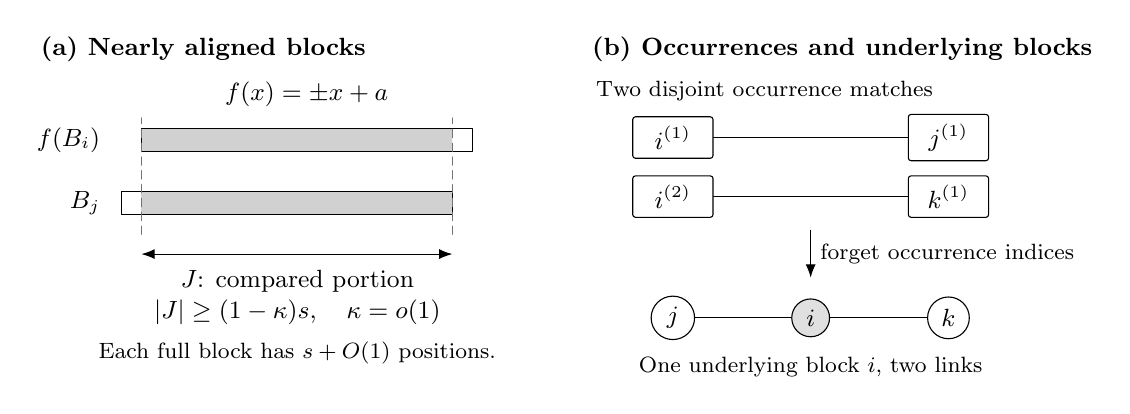
\begin{tikzpicture}[x=1cm,y=1cm,font=\small,
  line cap=round,line join=round,>=Latex]
  \node[anchor=west,font=\small\bfseries] at (0,4.05)
    {(a) Nearly aligned blocks};
  \node at (3.50,3.48) {$f(x)=\pm x+a$};
  \fill[black!18] (1.40,2.75) rectangle (5.35,3.05);
  \fill[black!18] (1.40,1.95) rectangle (5.35,2.25);
  \draw (1.40,2.75) rectangle (5.60,3.05);
  \draw (1.15,1.95) rectangle (5.35,2.25);
  \node[anchor=east] at (1.00,2.90) {$f(B_i)$};
  \node[anchor=east] at (1.00,2.10) {$B_j$};
  \draw[densely dashed,black!55] (1.40,1.70) -- (1.40,3.18);
  \draw[densely dashed,black!55] (5.35,1.70) -- (5.35,3.18);
  \draw[<->] (1.40,1.45) -- (5.35,1.45);
  \node[align=center] at (3.38,0.90)
    {$J$: compared portion\\$|J|\ge(1-\kappa)s,\quad\kappa=o(1)$};
  \node[font=\footnotesize,align=center] at (3.38,0.20)
    {Each full block has $s+O(1)$ positions.};

  \node[anchor=west,font=\small\bfseries] at (7.00,4.05)
    {(b) Occurrences and underlying blocks};
  \node[anchor=west,font=\footnotesize] at (7.05,3.52)
    {Two disjoint occurrence matches};
  \node[draw,rounded corners=1pt,minimum width=1.02cm,
    minimum height=0.48cm] (i1) at (8.15,2.93) {$i^{(1)}$};
  \node[draw,rounded corners=1pt,minimum width=1.02cm,
    minimum height=0.48cm] (j1) at (11.65,2.93) {$j^{(1)}$};
  \node[draw,rounded corners=1pt,minimum width=1.02cm,
    minimum height=0.48cm] (i2) at (8.15,2.18) {$i^{(2)}$};
  \node[draw,rounded corners=1pt,minimum width=1.02cm,
    minimum height=0.48cm] (k1) at (11.65,2.18) {$k^{(1)}$};
  \draw (i1) -- (j1);
  \draw (i2) -- (k1);
  \draw[->] (9.90,1.75) -- (9.90,1.15)
    node[midway,right,font=\footnotesize] {forget occurrence indices};
  \node[draw,circle,inner sep=2.5pt] (j) at (8.15,0.64) {$j$};
  \node[draw,circle,inner sep=2.5pt,fill=black!12] (i) at (9.90,0.64) {$i$};
  \node[draw,circle,inner sep=2.5pt] (k) at (11.65,0.64) {$k$};
  \draw (j) -- (i) -- (k);
  \node[font=\footnotesize] at (9.90,0.02)
    {One underlying block $i$, two links};
\end{tikzpicture}
\caption{Aligned blocks and the two levels of comparison.  In (a), away
from subcomparison ends, the image of a full grid interval is displaced
by $o(s)$ from a partner grid interval; the shaded portion $J$ records a
comparison of $s-o(s)$ positions.  Reflection reverses order and inverts
letters.  The intervals and their small end discrepancies are schematic.
In (b), $i^{(r)}$ denotes the $r$th occurrence of block $i$.  Occurrence
joins form a partial matching, but forgetting the occurrence indices
can give several links at one underlying block.}
\label{fig:aligned-blocks}
\end{figure}


\begin{lemma}\label{lem:link-word-counts}
There is a number $\rho_L\to0$, uniform over patterns, with the following
properties.  Every word assignment counted in this lemma is required
to be reduced on each block.
\begin{enumerate}
 \item Given the reduced word on one block of a link component
 $\mathcal U$, at most $\exp(\rho_Ls|\mathcal U|)$ assignments of
 words to all its blocks satisfy the link constraints.
 \item If $\mathcal U$ contains a self-link, the total number of such
 assignments is at most $\exp(\rho_Ls|\mathcal U|)$.
 \item If $\mathcal U$ has no self-link, then
 \begin{equation}\label{eq:component-multiplicity}
  2z_{\mathcal U}\leq S_{\mathcal U}+b_{\mathcal U}.
 \end{equation}
\end{enumerate}
\end{lemma}

\begin{proof}
Root a spanning tree of the link component at the block whose word is
given.  A link from a known block determines at least $(1-\kappa)s$
letters of the next block, whose total length is at most $s+1$.
There are at most $|T|^{\kappa s+1}$ choices for its remaining letters.
Multiplying along the tree proves the first assertion, even if we
ignore reducedness and all links outside the tree when making this
upper bound.

For the second assertion, start with a block carrying a self-link.
If its coordinate map is a translation, the constraint takes the form
$t_x=t_{x+a}$ on at least $(1-\kappa)s$ consecutive positions.  The
integer $a$ is nonzero: $a=0$ would pair occurrences of the same
underlying edge, violating \eqref{eq:distinct-comparison-edges}.
The equality graph on the $h_i$ positions is a forest.  In fact all its
edges have the same nonzero step, and within each residue class modulo
$|a|$ they connect successive positions in their natural order.
There are at least $(1-\kappa)s$ distinct equality edges, leaving at
most $h_i-(1-\kappa)s\leq\kappa s+1$ components.  Choosing one letter
per component gives at most $|T|^{\kappa s+1}$ choices.

A reflection self-link cannot occur with reduced block words.  Let
$J$ be the interval of positions on which the constraint reads
$t_x=\overline{t_{a-x}}$.  Its reflected image also lies in the same
block, and both have more than half the block's positions.
Their intersection is therefore a nonempty interval invariant under
reflection.  If it has a central fixed position, the letter there
would equal its inverse, contrary to the fixed-point-free involution
on $T$.  If it has no fixed position, its two central adjacent positions
are reflections of each other and have inverse letters, contrary to
reducedness.  After counting the words on the initial self-linked
block, propagate along a spanning tree as above.  Enlarging $\rho_L$
by a fixed factor proves the second assertion.

Finally, choose a block with $m_i=z_{\mathcal U}$.  If there is no
self-link, every matched occurrence of this block has its partner
among the $S_{\mathcal U}-z_{\mathcal U}$ occurrences of other blocks.
There are at least $z_{\mathcal U}-b_{\mathcal U}$ such matched
occurrences, and distinct occurrences have distinct partners.  Hence
$z_{\mathcal U}-b_{\mathcal U}\leq
S_{\mathcal U}-z_{\mathcal U}$, which is
\eqref{eq:component-multiplicity}.
\end{proof}

\subsection{Word bins and stage expectations}

The link constraints make the number of free words small.  To combine
this fact with the probability of embedding a labelled graph, we must
also retain each block's word weight.  For its word $W_i$, in the chosen
chain orientation, record the integer
\[
 d_i:=\lfloor-\log P(W_i)\rfloor.
\]
All these words are reduced.  Since the fixed collection of positive
turn weights has a positive minimum, there is a constant $a_0>0$
depending only on those weights such that, for large $L$,
\begin{equation}\label{eq:word-bin-bounds}
 \frac{\delta s}{2}\leq d_i\leq a_0s,
 \qquad
 \#\{W\in T^{h_i}:\lfloor-\log P(W)\rfloor=d_i\}
 \leq\exp(2d_i-\delta s).
\end{equation}
Here and below only positive-weight words are counted.  For completeness,
Lemma~\ref{lem:word-decay} implies
$P(W)^2\leq e^{-2\delta h_i}$ for each word, so
$d_i\geq\delta h_i-1\geq\delta s/2$ for large $s$.
The minimum turn weight gives the upper bound.  Every word in the bin
has $P(W)>e^{-d_i-1}$, and therefore the number in the bin is at most
\[
 e^{2d_i+2}\sum_{W\in T^{h_i}}P(W)^2
 \leq e^{2d_i+2-2\delta h_i}
 \leq e^{2d_i-\delta s}.
\]
These estimates are uniform because $h_i=s+O(1)$ and $s\to\infty$.

Enlarge the pattern by recording all $d_i$.  There are $O(L/s)$ full
blocks, each with $O(s)$ possible bins.  Thus the logarithm of the
number of bin choices is
$O((L/s)\log(s+2))=o(L)$.  Together with the earlier polynomial count,
the total number of enlarged patterns is
\begin{equation}\label{eq:pattern-entropy}
 \exp(o(L)).
\end{equation}
The grid, occurrence matching, and link multigraph are determined
by the unlabelled pattern, and introduce no further choices.

Fix one enlarged pattern.  A full label assignment means labels on
all edges of its abstract image graph, read inversely on reverse
edges, giving an immersion into $F$ and satisfying the comparisons
and bins.  This is a condition on strings on the abstract graph; it
does not require an embedding in the random graph.  At stage $j$,
consider the restrictions of all such full label assignments to
$\Delta_j$.  Let $Z_j$ count their injective realizations in $\Gamma$,
with the component sides prescribed by the pattern, and with the
root fixed if $k_j=1$.  Every realization of the original enlarged
pattern gives $Z_j\geq1$ at every stage.

For a fixed one of these stage label assignments, the expected number
of its realizations is at most
\begin{equation}\label{eq:fixed-stage-expectation}
 n^{V_j-E_j-k_j}
 \exp\left(-\sum_{i:m_i\geq j}d_i+o(L)\right).
\end{equation}
To prove this, let $Q_j$ be the number of active chains, that is,
chains whose edges belong to $\Delta_j$.  They have exactly
$E_j-Q_j$ unmarked internal vertices.  At such a vertex the incoming
and outgoing chain labels form a reduced turn $t,u$, and
\eqref{eq:turn-count} bounds its possible images on its prescribed side
by
\[
 np\,w(t,u)+O(1)=np\,w(t,u)(1+O(1/n)).
\]
At each remaining unfixed vertex use the upper bound $n$; a fixed root
is marked and has only one choice.  This bounds the number of possible
vertex assignments by
\[
 n^{V_j-k_j}p^{E_j-Q_j}
 \prod_{\text{internal turns of active chains}}w(t,u)
 \exp(O(L/n)).
\]
Restrict to the assignments that are injective and compatible with all
vertex types.  Each requires $E_j$ distinct edge prescriptions.
Lemma~\ref{lem:prescriptions} bounds their joint probability by
$(np)^{-E_j}\exp(o(L))$.  Multiplication leaves
$n^{V_j-E_j-k_j}p^{-Q_j}$ times the displayed turn product.
The bounded factor $p^{-Q_j}$ is $\exp(o(L))$.  Every turn weight is
at most one, so discarding all factors except internal turns of full
blocks increases the product.  The remaining product is
\[
 \prod_{i:m_i\geq j}P(W_i)
 \leq\exp\left(-\sum_{i:m_i\geq j}d_i\right),
\]
which proves \eqref{eq:fixed-stage-expectation}.  This count uses
injective realizations of the image graph; it does not replace distinct
edge prescriptions by repeated traversals.

The number of stage label assignments has the bound
\begin{equation}\label{eq:stage-label-count}
 \exp\left(o(L)+
 \sum_{\substack{\mathcal U\text{ without self-link}\\
                  z_{\mathcal U}\geq j}}
 \left(2\min_{i\in\mathcal U}d_i-\delta s\right)\right).
\end{equation}
Indeed, a link component is represented at stage $j$ exactly when
$z_{\mathcal U}\geq j$.  The possible words on its represented blocks
are projections of assignments on the entire link component.  A
projection has cardinality no larger than the set being projected.
If the component has no self-link, choose a block attaining the
minimum bin, even when that block is absent from stage $j$.
Equation~\eqref{eq:word-bin-bounds} gives at most
$\exp(2\min_i d_i-\delta s)$ choices on this block, and
Lemma~\ref{lem:link-word-counts} bounds the extensions by
$\exp(\rho_Ls|\mathcal U|)$.  If the component has a self-link,
the second assertion of that lemma gives this last factor without
any initial word choice.  Constraints between different words, or at
chain junctions, can only reduce these counts.

Summed over components, the propagation error is
$\rho_Ls\,O(L/s)=o(L)$.  There are only boundedly many chain end
fragments, containing $O(s)$ positions in total; assigning their
letters freely costs at most $|T|^{O(s)}=\exp(o(L))$.
These observations prove \eqref{eq:stage-label-count}.  Requiring
stage labels to extend as strings was essential: it permits the
minimum-bin block to be used even at stages where it is absent.

Let $B_j$ be the product of the right sides of
\eqref{eq:fixed-stage-expectation} and
\eqref{eq:stage-label-count}, choosing their uniform error bounds.
Then
\begin{equation}\label{eq:stage-markov}
 \mathbb E_L Z_j\leq B_j,
 \qquad
 \mathbb P_L(\text{the enlarged pattern is realized})
 \leq\min_{1\leq j\leq m_*}B_j.
\end{equation}
The second inequality is Markov's inequality at each individual stage.
We will now bound the minimum by multiplying the deterministic numbers
$B_j$.

\subsection{Combining the stages}

\begin{proof}[Proof of Theorem~\ref{thm:bounded-patterns}]
Lemma~\ref{lem:multiplicity-incidence} shows that the total exponent of
$n$ in $\prod_{j=1}^{m_*}B_j$ is nonpositive. For a component
$\mathcal U$ without a self-link, write
$d_{\min}=\min_{i\in\mathcal U}d_i$.  Its positive label-count term
occurs at $z_{\mathcal U}$ stages; the negative term $-d_i$ occurs at
$m_i$ stages.  Its total contribution to the logarithm, apart from
the uniform errors, is at most
\begin{align*}
 z_{\mathcal U}(2d_{\min}-\delta s)
       -\sum_{i\in\mathcal U}m_i d_i
 &\leq (2z_{\mathcal U}-S_{\mathcal U})d_{\min}
                -\delta s z_{\mathcal U}\\
 &\leq a_0s b_{\mathcal U}
                -\frac{\delta s}{2}S_{\mathcal U}.
\end{align*}
For the last inequality, if $2z_{\mathcal U}-S_{\mathcal U}\leq0$,
use $d_{\min}\geq\delta s/2$ to bound the preceding line by
$-\delta s S_{\mathcal U}/2$.  If
$2z_{\mathcal U}-S_{\mathcal U}>0$, use
$d_{\min}\leq a_0s$ and
$2z_{\mathcal U}-S_{\mathcal U}\leq b_{\mathcal U}$ from
\eqref{eq:component-multiplicity}; the remaining term satisfies
$-\delta s z_{\mathcal U}\leq-\delta s S_{\mathcal U}/2$.

For a component with a self-link there is no positive label-count
term, and \eqref{eq:word-bin-bounds} gives
\[
 -\sum_{i\in\mathcal U}m_i d_i
 \leq-\frac{\delta s}{2}S_{\mathcal U}.
\]
The full-block occurrences account for all positions except $O(s)$
positions in end fragments.  Replacing their actual lengths
$h_i=s+O(1)$ by $s$ changes the count by $O(L/s)$, because the
multiplicities are bounded.  Thus
\[
 s\sum_{\mathcal U}S_{\mathcal U}=H+O(s+L/s)=H+o(L).
\]
Equation~\eqref{eq:block-unmatched-budget} also gives
$s\sum_{\mathcal U}b_{\mathcal U}\leq b_0+o(L)$.
There are at most $M$ stages, so summing their uniform errors still
gives $o(L)$.  We conclude that
\begin{equation}\label{eq:stage-product}
 \log\prod_{j=1}^{m_*}B_j
 \leq-\frac\delta2 H+a_0b_0+o(L).
\end{equation}

Choose, once and for all,
\begin{equation}\label{eq:epsilon-choice}
 \varepsilon:=\min\left\{\frac14,
                  \frac{\delta}{16(1+a_0)}\right\}.
\end{equation}
Both $\delta$ and $a_0$ depend only on the fixed alphabet and weights,
so this choice is independent of $K_0,C,I$.  If $b_0\leq\varepsilon H$
and $H\geq L$, the uniform error in \eqref{eq:stage-product} is small
enough, for all sufficiently large $n$, that
\[
 \log\prod_{j=1}^{m_*}B_j\leq-\frac\delta4H.
\]
Some stage therefore has
\[
 B_j\leq\exp\left(-\frac{\delta H}{4m_*}\right)
       \leq\exp\left(-\frac{\delta H}{4M}\right).
\]
Equation~\eqref{eq:stage-markov} bounds the realization probability
of this enlarged pattern by the last expression.  No independence of
the stages has been used; a full realization must survive every one
of their separate first-moment bounds.  Finally, sum over the
$\exp(o(L))$ enlarged patterns from \eqref{eq:pattern-entropy} and
use $H\geq L$.  The resulting bound
\[
 \exp\left(-\frac{\delta L}{4M}+o(L)\right)
 \longrightarrow0
\]
proves the theorem, with the stated order of quantifiers.
\end{proof}

\section{From spherical arrangements to bounded path systems}
\label{sec:planar}

Theorem~\ref{thm:bounded-patterns} excludes path systems whose number of
paths, total length in units of $L$, and number of comparison intervals
are bounded.  The topological argument will produce a planar pairing of
paths with none of those bounds.  We show that every such pairing
yields a system covered by the theorem.  Planarity has two roles: an
Euler characteristic count organizes the pairing into few intervals,
and a separator reduces the number of paths while losing few paired
positions.  This is the spherical-arrangement method of
\cite[Section ``From bounded patterns to spherical arrangements'']{OpenAI2026ZD};
we include the geometric and quantitative details needed here.

\begin{definition}[Reduced spherical arrangement]
\label{def:reduced-arrangement}
A \emph{reduced spherical arrangement over $\Gamma$} consists of
finitely many pairwise disjoint piecewise linear closed disks in an
oriented sphere, together with the following data.
Each boundary reads a positive-length cyclically immersed closed path
in $\Gamma$, except possibly one boundary.  That boundary reads a
positive-length immersed interval path starting at $x_A$ or $x_B$,
with its two endpoints represented at a single marked boundary point,
called the \emph{break}.  No immersion condition is imposed across the
break.  At least one ordinary, cyclically immersed boundary is required.

The paths are read in the boundary orientations induced by the disks.
Their edge occurrences are paired in distinct twos by mutually disjoint
piecewise linear arcs.  The interiors of the arcs lie outside the disks,
and each occurrence contains exactly one arc endpoint in its interior.
Paired occurrences have inverse signed letters and use distinct
underlying undirected edges of $\Gamma$.
\end{definition}

The distinction between occurrences and graph edges is essential:
different occurrences may traverse the same edge, but the two ends of
any one pairing arc may not.  The graph obtained by collapsing each
disk to a vertex may be disconnected and may have loops or parallel
edges.

Proposition~\ref{prop:cone-criterion} will show that the absence of
these arrangements makes the cone complex aspherical and protects the
two roots. The present section proves that the random graphs can be
chosen to have this absence property.

\begin{theorem}[Absence of reduced spherical arrangements]
\label{thm:no-arrangements}
In the random matching model of Section~\ref{sec:random}, conditioned
on girth at least $L$, the probability that $\Gamma$ admits a reduced
spherical arrangement tends to zero as $m\equiv1\pmod4$ tends to
infinity.  Consequently, for every sufficiently large admissible $m$
there is a matching outcome with girth at least $L$, the component
diameter bound of Proposition~\ref{prop:diameter}, and no reduced
spherical arrangement.
\end{theorem}

We first establish the three deterministic tools used in the proof.
The first closes path segments without changing any original
occurrences.  The other two depend only on planarity.

\subsection{Closing immersed segments}

Fix the constant $d$ of Proposition~\ref{prop:diameter}, and work for
now with an outcome in which every component of $\Gamma$ has diameter
at most $dL$.  Each side of $\Gamma$ has at most $n$ vertices and minimum
degree at least $129$.

\begin{lemma}[Short closures]
\label{lem:closure}
There is a fixed integer $D_0$, depending only on $d$ and $c_0$, with
the following property for all sufficiently large admissible $n$.
If every component of $\Gamma$ has diameter at most $dL$, then every
positive-length immersed path segment in $\Gamma$ extends to a
cyclically immersed closed path by appending at most $D_0L$ edges.
The original segment is retained without cancellation.  One may take
any integer
\[
 D_0\ge d+\frac{8}{c_0\log2}+8.
\]
\end{lemma}

\begin{proof}
We first construct a short based loop that avoids specified edges at
its basepoint.  For large $n$ we have $L\ge3$, so the girth condition
excludes loops and parallel edges.  Delete at most two prescribed
undirected edges incident to a vertex $z$.  In the remaining graph
every vertex still has degree at least $127$, and in particular at
least three.  With
\[
 k=\lceil\log_2n\rceil+1,
\]
there are at least $3\cdot2^{k-1}>n$ non-backtracking walks of length
$k$ starting at $z$.  Two distinct such walks, say $P$ and $Q$, end
at the same vertex.  Reduce $PQ^{-1}$ as a linear path.  Cancellation
removes their common terminal segment.  Since $P$ and $Q$ are distinct
and have equal length, it does not remove either entire walk.  We
obtain a nonempty linearly immersed based loop of length at most $2k$;
its first and last edges avoid the deleted edges.  The loop need not
be cyclically immersed at $z$.

Let the given segment $S$ run from $a$ to $b$, and choose a geodesic
$R$ from $b$ to $a$, of length at most $dL$.  If $R$ is nonempty,
construct a loop $J_b$ at $b$ avoiding the last edge of $S$ and the
first edge of $R$, and a loop $J_a$ at $a$ avoiding the last edge of
$R$ and the first edge of $S$.  Then
\[
 S J_b R J_a
\]
is cyclically immersed: each constituent is immersed as a linear path,
and each of the four joins avoids immediate reversal.  If $R$ is empty,
then $a=b$, and one loop at $a$ avoiding the first and last edges of
$S$ makes $SJ_a$ cyclically immersed.  Thus the total added length is
at most $dL+4k$ in either case.  Finally,
$L\ge(c_0/2)\log n$ and $L\ge1$ for large $n$, so
\[
 k\le\left(\frac{2}{c_0\log2}+2\right)L.
\]
This gives the stated choice of $D_0$.
\end{proof}

\subsection{Organizing the pairing into intervals}

We next count how often a planar pairing can change its consecutive
partner interval.  A pair of neighboring arc ends usually has another
neighboring pair opposite it across a digon.  Only the other gaps,
and the places where we choose to split a path, require interval cuts.
This is the linear comparison-interval argument of
\cite[Lemma~4.3]{OpenAI2026ZD}.

\begin{lemma}[Paired intervals]
\label{lem:paired-intervals}
Suppose a reduced spherical arrangement with $N_0$ disk boundaries is
divided into $N'\ge N_0$ pieces by cutting its paths into consecutive
segments.  An intact path counts as one piece, and no piece crosses
the exceptional break.  Then all original occurrence pairings can be
represented by at most $6N'$ disjoint pairs of intervals.  Each interval
is contained in one designated piece, and each pair compares inverse
strings in reverse boundary order.  The intervals can also be required
not to cross one prescribed indexing gap between occurrences on each
original path, using the break as the exceptional indexing gap.
\end{lemma}

\begin{proof}
Thicken the disks and the pairing arcs to a closed regular neighborhood
$R$ made of disks and rectangular bands.  Write $E$ for the number of
bands, or equivalently the number of pairing arcs.  A \emph{gap} is the
portion of an original disk boundary between successive arc ends in
cyclic order.  After thickening, each gap gives a corner of a
complementary region.  For each connected component $Q$ of
$S^2\setminus\operatorname{int}R$, let $\ell_Q$ be the number of band
sides along its boundary, counting incidences.  This is also its number
of gap incidences.  Every disk has positive boundary length and every
occurrence is paired, so every boundary component of $R$ encounters a
band and $\ell_Q\ge1$.

The neighborhood $R$ retracts to the graph with $N_0$ vertices and $E$
edges.  Additivity of Euler characteristic when surfaces are glued
along boundary circles therefore gives
\[
 \chi(R)=N_0-E,\qquad
 \sum_Q\chi(Q)=2-N_0+E,\qquad
 \sum_Q\ell_Q=2E.
\]
In particular,
\begin{equation}
 \sum_Q\bigl(\ell_Q-2\chi(Q)\bigr)=2N_0-4.
 \label{eq:arrangement-euler}
\end{equation}
This identity does not require $R$ to be connected; the regions $Q$
may have several boundary components.

Call a gap \emph{good} if its region $Q$ is a disk digon whose two sides
belong to distinct bands.  The two corners of such a digon are opposite
good gaps.  Figure~\ref{fig:good-digon} shows how coherent boundary
orientations reverse the order of occurrences across such a digon.

\begin{figure}[tbp]
\centering
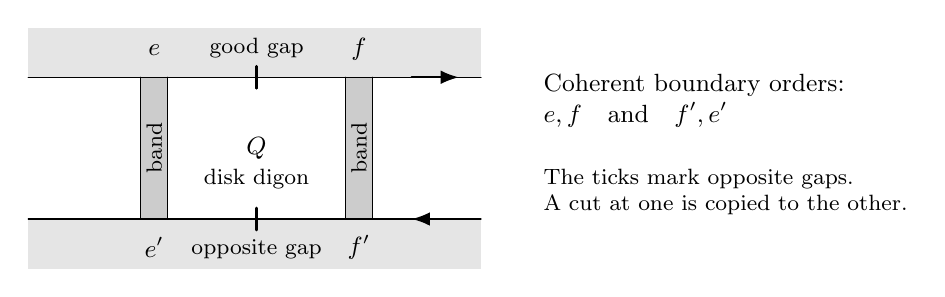
\begin{tikzpicture}[x=1cm,y=1cm,font=\small,
  line cap=round,line join=round,>=Latex]
  \fill[black!10] (0.60,2.20) rectangle (6.35,2.83);
  \fill[black!10] (0.60,-0.23) rectangle (6.35,0.40);
  \fill[black!20] (2.03,0.40) rectangle (2.37,2.20);
  \fill[black!20] (4.63,0.40) rectangle (4.97,2.20);
  \draw (0.60,2.20) -- (6.35,2.20);
  \draw (0.60,0.40) -- (6.35,0.40);
  \draw (2.03,0.40) -- (2.03,2.20);
  \draw (2.37,0.40) -- (2.37,2.20);
  \draw (4.63,0.40) -- (4.63,2.20);
  \draw (4.97,0.40) -- (4.97,2.20);
  \draw[->,line width=0.8pt] (5.47,2.20) -- (6.07,2.20);
  \draw[->,line width=0.8pt] (6.07,0.40) -- (5.47,0.40);
  \node at (2.20,2.55) {$e$};
  \node at (4.80,2.55) {$f$};
  \node at (2.20,0.04) {$e'$};
  \node at (4.80,0.04) {$f'$};
  \node at (3.50,1.30) {$Q$};
  \node[font=\footnotesize] at (3.50,0.91) {disk digon};
  \draw[line width=1pt] (3.50,2.06) -- (3.50,2.34);
  \draw[line width=1pt] (3.50,0.26) -- (3.50,0.54);
  \node[font=\footnotesize] at (3.50,2.57) {good gap};
  \node[font=\footnotesize] at (3.50,0.02) {opposite gap};
  \node[font=\footnotesize,rotate=90] at (2.20,1.30) {band};
  \node[font=\footnotesize,rotate=90] at (4.80,1.30) {band};
  \node[align=left,anchor=west] at (7.02,1.90)
    {Coherent boundary orders:\\$e,f$\quad and\quad $f',e'$};
  \node[align=left,anchor=west,font=\footnotesize] at (7.02,0.74)
    {The ticks mark opposite gaps.\\A cut at one is copied to the other.};
\end{tikzpicture}
\caption{A good gap and its opposite gap, shown locally between two
distinct bands.  The complementary region $Q$ is a disk digon.  The
coherent boundary orientations reverse the order of the paired
occurrences: $e,f$ on one boundary correspond to $f',e'$ on the other.
Thus an indexing or splitting cut at a good gap must also cut its
opposite gap, so that the remaining runs pair as whole intervals.
The symbols denote occurrences, not underlying edges of $\Gamma$;
shading only distinguishes disk portions and bands in the surface.}
\label{fig:good-digon}
\end{figure}


Let $B$ be the number of gaps that are not good.  We bound $B$ by
treating the possible complementary regions as follows.

A disk monogon has one gap between two occurrences joined by the same
pairing arc.  Those neighboring letters are inverse.  Immersion rules
this out except at the exceptional break, so the number $M$ of disk
monogons is at most one.  Their total contribution to
Equation~\ref{eq:arrangement-euler} is $-M$.

A disk digon using the same band twice turns immediately back along
that band at an endpoint.  The associated gap is the sole gap at a
disk with only one incident arc end: otherwise another band end would
intervene in its cyclic order.  Different such digons use different
degree-one gaps.  Hence there are at most $N_0$ such digons and at
most $2N_0$ gaps on them.

Every remaining region is either a disk with $\ell_Q\ge3$, or a
connected planar surface with at least two boundary components.  In
the first case $\ell_Q\le3(\ell_Q-2)$; in the second case
$\chi(Q)\le0$, and the stronger inequality
$\ell_Q\le\ell_Q-2\chi(Q)$ holds.  These regions have positive
contributions to Equation~\ref{eq:arrangement-euler}, with total
$2N_0-4+M$.  Digons contribute zero.  It follows that
\begin{equation}
 B\le M+2N_0+3(2N_0-4+M)\le8N_0.
 \label{eq:non-good-gaps}
\end{equation}

Across a good digon, the partners of consecutive occurrences $e,f$
occur consecutively in the opposite order $f',e'$.  Taking opposite
corners is thus an involution on good gaps.  Cut every original
boundary at every non-good gap.  Also mark its prescribed indexing
gap, using the break on the exceptional boundary, and mark all gaps
used in dividing the paths into the designated pieces.  These extra
marks number at most $N_0+N'$.  For each marked good gap, cut both it
and its opposite gap.  The resulting cut set is stable under the
good-gap involution, and its cardinality $J$ satisfies
\[
 J\le B+2(N_0+N')\le12N'.
\]

Every boundary has a cut, so the remaining consecutive runs of
occurrences are linear intervals.  All of them lie within designated
pieces.  Pairing reverses each uncut adjacency, and stability of the
cuts ensures that it takes a whole maximal run onto another whole
maximal run.  A run cannot be paired with itself.  For an odd-length
run this would fix its middle occurrence, whereas occurrences are
paired in distinct twos.  For an even-length run it would pair the
two middle occurrences and make their adjacent letters inverse.
That contradicts immersion inside the run; the exceptional break has
been cut.  The $J$ runs therefore pair in distinct twos, giving at most
$J/2\le6N'$ interval pairs as claimed.
\end{proof}

\subsection{A recursive separator bound}

Once a long boundary has been divided into pieces of controlled
length, deleting a small fraction of the pieces loses only a small
fraction of all occurrences.  The following consequence of the planar
separator theorem, also used in \cite[Lemma~4.4]{OpenAI2026ZD}, makes
the remaining groups of pieces bounded in size.

\begin{lemma}[Recursive planar separation]
\label{lem:separator}
Let
\[
 C_{\mathrm{sep}}=\frac{2\sqrt2}{1-\sqrt{2/3}}.
\]
For every integer $K_0\ge1$, a finite planar multigraph with $N'$
vertices has a set of at most $C_{\mathrm{sep}}N'/\sqrt{K_0}$ vertices
whose deletion leaves every connected component with at most $K_0$
vertices.
\end{lemma}

\begin{proof}
Deleting loops and replacing parallel edges by single edges preserves
the components after every possible vertex deletion, so it suffices
to consider a simple planar graph.  The Lipton--Tarjan separator theorem
\cite{LiptonTarjan1979} gives, for a simple planar graph on $s$ vertices,
a set of at most $2\sqrt{2s}$ vertices whose removal leaves components
with at most $2s/3$ vertices.  Apply this theorem recursively to each
component with more than $K_0$ vertices, starting separately on the
original connected components.

At a recursive call on $s>K_0$ vertices, charge each of those vertices
$2\sqrt2/\sqrt{s}$.  The total charge at that call is $2\sqrt{2s}$ and
bounds the number of vertices removed there.  Follow any fixed original
vertex through the calls containing it, until it is deleted or belongs
to a component of size at most $K_0$.  The successive charged component
sizes decrease by a factor at most $2/3$.  Reading backwards from the
last charged size, which is greater than $K_0$, bounds its total charge
by
\[
 \frac{2\sqrt2}{\sqrt{K_0}}
 \sum_{j\ge0}(2/3)^{j/2}
 =\frac{C_{\mathrm{sep}}}{\sqrt{K_0}}.
\]
This applies also to a vertex deleted by a separator.  Summing the
charges over all $N'$ original vertices bounds the total number
deleted and proves the lemma.
\end{proof}

\subsection{Extracting one bounded path system}

We now combine these tools.  The original paths will first be divided
and closed, then separated into clusters.  We retain a cluster whose
proportion of unpaired occurrences and number of interval pairs are
both small.  Controlling the total losses, rather than those of every
cluster, is enough to find one such cluster.

\begin{proof}[Proof of Theorem~\ref{thm:no-arrangements}]
Let $\varepsilon>0$ be the constant in
Theorem~\ref{thm:bounded-patterns}, independent of its fixed bounds
$K_0,C,I$.  Fix $d$ from Proposition~\ref{prop:diameter} and $D_0$ from
Lemma~\ref{lem:closure}. We will cut long boundaries into pieces with
at most $UL$ original occurrences, pay at most $D_0L$ to close each
cut piece, and delete at most an $\eta$ fraction of the pieces.
We choose $U$ large enough to make the closure overhead small and
$\eta$ small enough to control the occurrences lost in separation.
Specifically, choose the following constants in order:
\begin{align}
 U&\ge\max\{3,\lceil96D_0/\varepsilon\rceil\},
       &&\text{$U$ an integer},\notag\\
 \eta&=\min\{1/(32U),\varepsilon/(64U)\},\qquad
 K_0=\max\{1,\lceil(C_{\mathrm{sep}}/\eta)^2\rceil\},
 \label{eq:extraction-constants}\\
 C&=K_0(U+D_0),\qquad I=\lceil192C\rceil.\notag
\end{align}
In particular,
\begin{equation}
 \frac{3D_0}{U}\le\frac{\varepsilon}{32},\qquad
 2\eta U\le\frac1{16},\qquad
 2\eta U\le\frac{\varepsilon}{32}.
 \label{eq:extraction-losses}
\end{equation}
All these constants are fixed before $n=vm$ tends to infinity through
$m\equiv1\pmod4$.  Their order of dependence is
\[
 (\text{types},c_0,\delta)\ ;\quad
 (\varepsilon,d)\ ;\quad D_0\ ;\quad U\ ;\quad\eta\ ;\quad
 K_0\ ;\quad (C,I)\ ;\quad n.
\]

Suppose there is a reduced spherical arrangement on an outcome
satisfying the diameter bound.  Let $N_0$ be its number of boundaries
and $H_0$ their total length.  An ordinary boundary is present, and
girth gives $H_0\ge L$.

Keep every path of length at most $UL$ intact.  For a longer path of
length $h$, put $r=\lceil h/(UL)\rceil$ and divide it into $r$
consecutive segments whose integer lengths differ by at most one.
For large $L$ each segment has length between $UL/3$ and $UL$:
$h/r>UL/2$, so $\lfloor h/r\rfloor\ge UL/3$ when $UL\ge6$, while
$\lceil h/r\rceil\le UL$.  Use the linear order from the root on an
exceptional path, so no segment crosses its break.  Close each segment
of every path that was split using Lemma~\ref{lem:closure}.  Every
newly appended occurrence is left unpaired; intact paths receive no
added edges.

Let $N'$ be the number of resulting paths, and let $H_{\mathrm{add}}$
be their total added length.  Each resulting path contains at most
$UL$ original occurrences and has total length at most $(U+D_0)L$.
Since a split path contributes at most $3h/(UL)$ pieces,
\begin{equation}
 H_{\mathrm{add}}\le\frac{3D_0}{U}H_0.
 \label{eq:added-length}
\end{equation}
Every piece has at least $L$ original occurrences, by girth for intact
ordinary paths and by $UL/3\ge L$ for split paths, except possibly the
one intact exceptional path.  Thus
\begin{equation}
 N_0\le N',\qquad N'L\le H_0+L\le2H_0.
 \label{eq:extraction-piece-count}
\end{equation}
If the exceptional path was split, all its pieces have become closed
cyclically immersed paths.  Otherwise it remains a single immersed
interval starting at its original root.

Apply Lemma~\ref{lem:paired-intervals} before the closures are appended.
The original pairing is specified by at most $6N'$ interval pairs,
each lying in its designated pieces.  Choose the indexing points of
intact ordinary paths as in that lemma; index every newly closed path
with its original segment followed by its closure.  The interval
comparisons therefore remain valid in the indexed resulting paths.

Form a multigraph whose vertices are the $N'$ pieces and whose edges
are the original pairing arcs.  It is planar: within each old disk,
replace its vertex by one vertex for each consecutive block of arc
ends belonging to a piece.  Each block can be connected to its new
vertex inside a separate sector of the disk.  This produces disjoint
connections, also for original arcs with both ends at the same disk.
The appended closures have no pairing arcs and play no role in this
embedding.

By Lemma~\ref{lem:separator} and the choice of $K_0$, delete at most
$\eta N'$ vertices, leaving components with at most $K_0$ pieces.
Call these components \emph{clusters}.  If $M_{\mathrm{del}}$ is the
number of original occurrences in deleted pieces, then
\begin{equation}
 M_{\mathrm{del}}\le\eta N'UL\le2\eta U H_0.
 \label{eq:deleted-occurrences}
\end{equation}
Keep an original pairing precisely when both of its pieces survive.
At most $M_{\mathrm{del}}$ surviving original occurrences lose their
partners, because each deleted occurrence had just one partner.
An interval pair is either wholly retained or wholly discarded:
each of its two intervals lies in one piece.  Every retained pair
belongs to a single cluster.

For each cluster $Z$, denote its total path length by $H_Z$, including
added closures, its number of unpaired occurrences by $b_Z$, and its
number of retained interval pairs by $I_Z$.  Equations~\ref{eq:added-length}--\ref{eq:deleted-occurrences}
and the parameter choices give
\begin{align}
 \sum_Z H_Z&\ge H_0-M_{\mathrm{del}}\ge15H_0/16,
 & H_Z&\le K_0(U+D_0)L=CL,\notag\\
 \sum_Z b_Z&\le M_{\mathrm{del}}+H_{\mathrm{add}}
                \le\varepsilon H_0/16,
 &\sum_Z I_Z&\le6N'\le12H_0/L.
 \label{eq:cluster-budgets}
\end{align}
These are totals over all remaining clusters; an individual cluster
need not yet satisfy the bounded-pattern conditions.

Discard all clusters with $b_Z>\varepsilon H_Z$.  Their total length
is at most $\varepsilon^{-1}\sum_Z b_Z\le H_0/16$.  Also discard all
clusters with $I_Z>192H_Z/L$.  Their total length is at most
$(L/192)\sum_Z I_Z\le H_0/16$.  After these two exclusions, at least
$13H_0/16$ of cluster length remains.

A cluster with $H_Z<L$ contains no positive-length cyclically immersed
path, by girth.  It can therefore consist only of the one intact
exceptional path.  There is at most one such cluster.  If its length
is $h<L$, the original arrangement also has an ordinary boundary of
length at least $L$, so $H_0\ge h+L>2h$.  Discarding this final cluster,
if present, costs less than $H_0/2$.  A positive total length remains,
since $13H_0/16-H_0/2=5H_0/16>0$.

Choose one remaining cluster.  It has at most $K_0$ positive-length
paths and satisfies
\[
 L\le H_Z\le CL,\qquad b_Z\le\varepsilon H_Z,\qquad
 I_Z\le192H_Z/L\le192C\le I.
\]
All paths are cyclically immersed except possibly the entire intact
exceptional interval, still starting at $x_A$ or $x_B$.  The retained
comparisons still pair distinct underlying edges.  Closures may
revisit edges or meet other paths, but their occurrences are all
unpaired, which Theorem~\ref{thm:bounded-patterns} permits.  This
cluster is therefore a path system excluded by that theorem for the
single fixed triple $(K_0,C,I)$ in
Equation~\ref{eq:extraction-constants}.

The construction applies to every finite arrangement, with no bound on
$N_0$ or $H_0$, and always yields a system for that same triple.
The probability of such a system is $o(1)$ by
Theorem~\ref{thm:bounded-patterns}; the probability that the diameter
bound fails is $o(1)$ by Proposition~\ref{prop:diameter}.  This proves
the asserted exclusion probability.  The simultaneous girth,
diameter, and exclusion requirements consequently have positive
probability for all sufficiently large admissible $m$.
\end{proof}

\section{Cone pictures, asphericity, and protected roots}\label{sec:topology}

The probabilistic argument has produced finite immersed graphs for which
no reduced spherical arrangement exists.  We now turn that exclusion
into the two geometric properties needed in Section~\ref{sec:algebra}:
asphericity of the cone complex and protection of the roots.  We give
the cone-picture argument of
\cite[Proposition~5.1 and Corollary~5.3]{OpenAI2026ZD} in full,
including the surgeries that
preserve a rooted boundary.

\begin{proposition}[Cone criterion]\label{prop:cone-criterion}
Let $\Gamma=\Gamma_A\sqcup\Gamma_B$ be a finite graph immersed in the
rose $F$, with chosen roots $x_A,x_B$, and let $X$ and $G$ be defined
by \eqref{eq:cone-complex}.  If $\Gamma$ admits no reduced spherical
arrangement as in Definition~\ref{def:reduced-arrangement}, then
\[
 \pi_2(X)=0
 \quad\text{and}\quad
 \text{the root-protection condition \eqref{eq:root-protection} holds}.
\]
Moreover, $X$ is a finite aspherical complex of dimension at most two,
and $G$ is finitely presented and torsion-free.
\end{proposition}

The main issue is to pass from a sphere or a null-homotopy to a reduced
arrangement.  Its disks will record fillings through cones, and its arcs
will record inverse letters in the intervening map to the rose.  When a
pair of inverse letters traverses the same edge of $\Gamma$, a band
surgery removes that pair.  Minimizing the total boundary length makes
all such pairs impossible.

\subsection{Maps represented by cone pictures}

For $\Sigma=S^2$ or $D^2$, a \emph{cone picture} is a map
$f\colon\Sigma\to X$ together with finitely many pairwise disjoint
piecewise linear closed disks $D_i$ in the interior of $\Sigma$ with
the following properties.  On the complement of their interiors, $f$
takes values in $F$.  For each $i$ there is a component $\Lambda_i$ of
$\Gamma$ and a factorization
\[
 f|_{D_i}\colon D_i\longrightarrow K_{\Lambda_i}\longrightarrow X
\]
whose restriction to $\partial D_i$ is a specified closed edge path
in $\Lambda_i$.  In the disk case we also specify an edge path in
$\Gamma$ whose label is read on $\partial\Sigma$.  That path may have
distinct endpoints, since all graph vertices map to $*$.

\begin{lemma}[Picture representation]\label{lem:cone-pictures}
Every map $S^2\to X$ is homotopic to a cone picture.  Every disk map
whose boundary is the label of a specified edge path in $\Gamma$ is
homotopic relative to that boundary to a cone picture.
\end{lemma}

\begin{proof}
We first give a relative replacement of each cone by ordinary relator
disks.  Choose a maximal tree in a component $\Lambda$ and a vertex of
that tree.  The edges outside the tree give a free basis of
$\pi_1(\Lambda)$, represented by based edge loops.  Let $Y_\Lambda$
be $\Lambda$ with one disk attached along each of these basis loops.
Van Kampen's theorem gives $\pi_1(Y_\Lambda)=0$.  The cellular boundary
map from its two-cells has image the integral cycle group of $\Lambda$
and is injective: the basis loops give a basis of
$H_1(\Lambda;\mathbb Z)$.  Therefore $Y_\Lambda$ has zero reduced
integral homology.  A simply connected acyclic CW complex is
contractible, by the Hurewicz and Whitehead theorems
\cite[Sections 4.1 and 4.2]{Hatcher2002}.

Both $Y_\Lambda$ and $K_\Lambda$ contain $\Lambda$ as a CW subcomplex
and are contractible.  The identity on $\Lambda$ extends to maps in
both directions: extend successively over the relative cells, using
the vanishing homotopy groups of the target.  The two composites are
homotopic to the corresponding identities relative to $\Lambda$.
For this last assertion use the same cell-extension argument on the
products with $[0,1]$, prescribing the homotopy on the two ends and on
$\Lambda\times[0,1]$.  Thus the replacements are homotopy equivalences
relative to $\Lambda$, not merely equivalences of their absolute
homotopy types.  After attachment along $\Lambda\to F$, they give a
homotopy equivalence relative to $F$ between $X$ and the finite
presentation complex obtained from $F$ by attaching these relator
disks.

Here is the picture construction for this presentation complex.
Replace the attaching maps by mapping-cylinder collars and subdivide,
so that simplicial approximation applies to the surface map.  This
changes neither the homotopy type relative to $F$ nor a prescribed
boundary word.  In the interior of each relator disk choose a point
outside the images of the one-dimensional simplices and of the
degenerate two-dimensional simplices of the surface.  Its preimage is
a finite set of points, each with a neighborhood mapped
homeomorphically to a neighborhood of the chosen point.  By compactness
and finiteness of the triangulations, a sufficiently small closed disk
about the chosen point has as its entire preimage a disjoint union of
such disk neighborhoods.

In each target relator disk, expand that small disk to the full disk
and collapse the surrounding annulus radially to its boundary.  This
map is homotopic to the identity relative to the boundary.  Collapse
the mapping-cylinder collars to their attaching paths in $F$ as well.
After postcomposition, the surface outside the selected source disks
maps into $F$, while each source disk maps into one relator disk.
Returning through the relative equivalence to $X$ makes each of these
disk maps factor through the corresponding abstract cone.  All
homotopies fix a prescribed outer boundary.  This gives the asserted
cone pictures.
\end{proof}

We shall also use two elementary changes to a picture.  A homotopy of
one inner boundary path in its graph can be made on a collar of that
boundary.  Fill the resulting boundary in the same cone.  The new and
old fillings, with the collar included, are homotopic relative to the
original boundary because the abstract cone is contractible.  Thus
inner paths can be tightened cyclically.  If the result is constant,
the inner disk can be removed, filling it by that constant map into
$F$.  An outer path can likewise be tightened with its graph endpoints
fixed; the corresponding homotopy of its label is accommodated by a
boundary collar.

\subsection{Length reduction by band surgery}

Suppose first that $\pi_2(X)\ne0$.  Among cone pictures representing
non-null-homotopic spheres, choose one minimizing the sum of the lengths
of its inner boundary paths.  Alternatively, suppose root protection
fails.  Fix a root $r\in\{x_A,x_B\}$ and a distinct vertex $z$ joined
to it by a path with trivial label in $G$.  Among all cone pictures of
null-homotopies of labels of paths from $r$ to this fixed $z$, choose
one minimizing the sum of all inner boundary lengths and the outer
path length.  These minima exist because lengths are nonnegative
integers and Lemma~\ref{lem:cone-pictures} provides the required
pictures.  Among pictures attaining the minimum, remove all constant
inner boundaries.

The preceding collar changes show that every remaining inner boundary
is nonempty and cyclically immersed.  In the disk case the outer path
is immersed and nonempty, since its endpoints are distinct.  There is
at least one inner disk.  For the sphere case, a map with no such disk
would factor through $F$, whose universal cover is a tree and whose
second homotopy group is zero.  For the disk case, a nonempty immersed
path in $\Gamma$ has a nonempty freely reduced label word, which
cannot bound a disk in $F$.

Complete a disk picture to a sphere by adjoining a formal exterior
disk $D_\infty$.  Its interior carries no map into $X$.  Mark its
boundary at the initial point of the specified outer path; this is
the exceptional break, representing the two endpoints of that path.
Choose the orientation of the sphere so that the boundary of
$D_\infty$, starting at the break, reads the path from $r$ to $z$.
This choice may reverse all ordinary boundary words, which preserves
cyclic immersion.  In the sphere case simply orient the sphere and
give all disks their induced orientations.

On the complement of these disks, the map takes values in the rose.
Put it in piecewise linear general position with respect to one point
in the interior of each rose edge, keeping the boundary words fixed.
The preimages of these points are disjoint embedded arcs and circles.
Every letter occurrence has exactly one arc endpoint.  Discard the
circles.  The arcs pair all occurrences, and paired letters are inverse
when read in the oriented disk boundaries: the two ends of a
transverse arc have opposite crossing signs, and disk-boundary
orientations are opposite to those of the complementary surface.

It remains to show that paired occurrences use distinct underlying
edges of $\Gamma$.  Suppose an arc pairs two traversals of the same
edge $e$.  Choose a thin rectangular band around the arc.  It maps
into a small open interval in the corresponding rose edge and lifts
to the interior of the abstract graph edge $e$.  The lift agrees with
both specified boundary lifts at the band ends.  Whenever an inner
disk meets the band, its cone must therefore be the cone on the
component containing $e$.

The local shortening is particularly simple in graph paths.  Splice
the disk boundaries along the two sides of the band and then contract
the residual portions of the two paired traversals within $e$.
This removes two full edge occurrences in total. For ordinary
boundaries the changes, with suitable cyclic starting points, are
\begin{equation}\label{eq:inner-surgery-words}
 (eP,\ e^{-1}Q)\longmapsto PQ,
 \qquad
 eP e^{-1}Q\longmapsto(P,Q).
\end{equation}
Here $e^{-1}$ denotes the reverse oriented graph edge, rather than
merely a letter with the same label.  Consequently all concatenations
in \eqref{eq:inner-surgery-words} are paths in the same graph, and the
new boundaries are closed.  For a rooted exterior boundary the
corresponding changes are
\begin{equation}\label{eq:exterior-surgery-words}
 (P e R,\ e^{-1}Q)\longmapsto PQR,
 \qquad
 P e Q e^{-1}R\longmapsto PR.
\end{equation}
In the second formula $Q$ is closed at the terminal vertex of $e$;
in both formulas the resulting exterior path has exactly the original
graph endpoints $r,z$.  The contractions along $e$ are realized by
boundary-collar homotopies.

We now specify the resulting surface maps in all four cases.  This
also explains why the operation retains the failure that was
minimized.

If the band joins two distinct inner disks, their union with the band
is a disk.  The maps on all three pieces factor together through the
same abstract cone, since their lifts agree on the attaching intervals.
Replace them by this single cone disk and shorten its boundary as in
the first formula of \eqref{eq:inner-surgery-words}.  The replacement
is homotopic to the old map relative to the rest of the surface, and
the total boundary length decreases by two.  Further tightening can
only decrease it.  An essential sphere remains essential, and a disk
still fills the same exterior word.

If the band joins an inner disk to $D_\infty$, their union is again a
disk, now an enlarged exterior disk.  Retain its complementary disk
and restrict the old map to that complement.  Its new boundary is
$PQR$ as in the first formula of \eqref{eq:exterior-surgery-words}.
The resulting picture is a null-homotopy of a path from $r$ to $z$;
the old inner boundary and exterior boundary have been replaced by a
boundary shorter than their combined length by two.

If both ends of the band lie on $D_\infty$, their union is an annulus
in the completed sphere.  Its complement consists of two disks.
Retain the one whose boundary contains the marked break, as shown
in Figure~\ref{fig:exterior-surgery}.  The restricted map on that disk,
after the edge-collar contraction, fills the word $PR$ in the second
formula of \eqref{eq:exterior-surgery-words}.  Thus this operation uses
only a restriction of the existing map; it does not require a
separate filling of $Q$.  It preserves the fixed endpoints and
decreases the total length by at least two.  The path $PR$ cannot
tighten to the empty path, because $r\ne z$.

\begin{figure}[H]
\centering
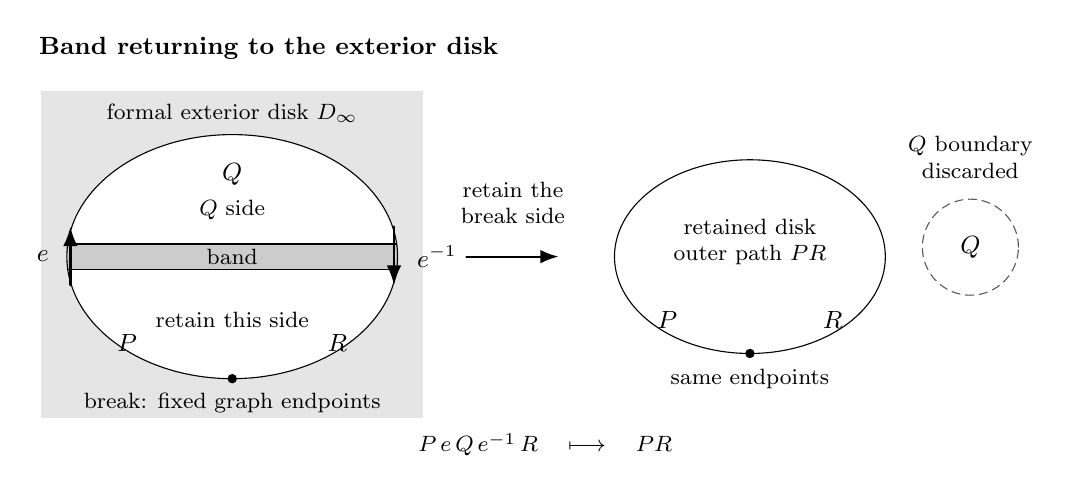
\begin{tikzpicture}[x=1cm,y=1cm,font=\small,
  line cap=round,line join=round,>=Latex]
  \node[anchor=west,font=\small\bfseries] at (0,3.00)
    {Band returning to the exterior disk};
  \fill[black!10] (0.15,-1.70) rectangle (5.00,2.45);
  \fill[white] (2.575,0.35) ellipse (2.10cm and 1.55cm);
  \fill[black!20] (0.475,0.19) rectangle (4.675,0.51);
  \draw (2.575,0.35) ellipse (2.10cm and 1.55cm);
  \draw (0.49,0.19) -- (4.66,0.19);
  \draw (0.49,0.51) -- (4.66,0.51);
  \node[font=\footnotesize] at (2.575,2.17)
    {formal exterior disk $D_\infty$};
  \node[font=\footnotesize,fill=black!20,inner sep=1pt]
    at (2.575,0.35) {band};
  \node at (2.575,1.40) {$Q$};
  \node[font=\footnotesize] at (2.575,0.94) {$Q$ side};
  \node at (1.24,-0.75) {$P$};
  \node at (3.91,-0.75) {$R$};
  \node[font=\footnotesize] at (2.575,-0.45) {retain this side};
  \draw[->,line width=0.9pt] (0.52,-0.01) -- (0.52,0.73);
  \draw[->,line width=0.9pt] (4.63,0.73) -- (4.63,-0.01);
  \node[anchor=east] at (0.37,0.35) {$e$};
  \node[anchor=west] at (4.80,0.35) {$e^{-1}$};
  \fill (2.575,-1.20) circle (1.7pt);
  \node[font=\footnotesize,align=center] at (2.575,-1.51)
    {break: fixed graph endpoints};

  \draw[->,line width=0.8pt] (5.55,0.35) -- (6.72,0.35);
  \node[font=\footnotesize,align=center] at (6.14,1.03)
    {retain the\\break side};

  \draw (9.15,0.35) ellipse (1.72cm and 1.23cm);
  \node[font=\footnotesize,align=center] at (9.15,0.54)
    {retained disk\\outer path $PR$};
  \node at (8.10,-0.45) {$P$};
  \node at (10.20,-0.45) {$R$};
  \fill (9.15,-0.88) circle (1.7pt);
  \node[font=\footnotesize] at (9.15,-1.20) {same endpoints};
  \node[font=\footnotesize,align=center] at (11.95,1.61)
    {$Q$ boundary\\discarded};
  \draw[densely dashed,black!65] (11.95,0.47) circle (0.61cm);
  \node at (11.95,0.47) {$Q$};
  \node[font=\footnotesize] at (6.55,-2.04)
    {$P\,e\,Q\,e^{-1}\,R\quad\longmapsto\quad PR$};

\end{tikzpicture}
\caption{A band returning to the formal exterior disk, shown
schematically in the domain sphere.  The two paired occurrences
traverse the same graph edge in opposite directions.  The exterior
disk and the band form an annulus.  Retaining its complementary disk
on the break side replaces $PeQe^{-1}R$ by $PR$ with the same graph
endpoints: $Q$ is closed at the terminal vertex of $e$, and the
restricted picture fills $PR$.  Shading denotes the formal exterior
disk and band; the exterior disk itself carries no map to $X$.}
\label{fig:exterior-surgery}
\end{figure}


Finally suppose both band ends lie on one inner disk.  The union $N$
of the disk and band is an annulus, and its map factors through the
same abstract cone $K_\Lambda$.  The complement of $N$ in the sphere
consists of two disks $Q_1,Q_2$.  Cap each new boundary by a disk
mapping through $K_\Lambda$, using the boundary lifts inherited from
$N$, and shorten these boundary paths to $P$ and $Q$ in the second
formula of \eqref{eq:inner-surgery-words}.  In the rooted case one of
$Q_1,Q_2$ contains $D_\infty$.  Retain that component with its new
cap and remove the formal exterior disk.  This is another disk
picture with the same exterior path.  Its total inner boundary length
is at most the old total minus two, because the two possible new cap
boundaries together have length two less than the old boundary and
all other retained disks already belonged to the old picture.

In the sphere case, the same operation gives two capped spheres; at
least one must still be essential.  To verify this without an
ambiguity from choices of caps, lift the original sphere map to the
universal cover $\widetilde X$.  The factorization $N\to K_\Lambda\to
X$ lifts through a single lift $K_\Lambda\to\widetilde X$, chosen to
agree with the lifted sphere on $N$.  Use that very same lift for
both new caps.  Write $\widetilde f_1,\widetilde f_2$ for the resulting
lifted capped spheres, with the orientations induced from $Q_1,Q_2$.
Their fundamental homology classes satisfy
\begin{equation}\label{eq:sphere-surgery-homology}
 \widetilde f_*[S^2]
   =\widetilde f_{1*}[S^2]+\widetilde f_{2*}[S^2]
       \quad\text{in }H_2(\widetilde X;\mathbb Z).
\end{equation}
Compute this identity before the boundary-collar shortenings, which
are homotopies and do not change these homology classes.  The
difference of the cycles on the two sides consists of the
old annulus and the two caps, with their boundary orientations
canceling.  This cycle factors through the contractible abstract cone
$K_\Lambda$, so its homology class is zero.  No assertion that the
image of this cone is an embedded contractible subspace is needed.
Since $\widetilde X$ is simply connected, the Hurewicz map
$\pi_2(\widetilde X)\to H_2(\widetilde X;\mathbb Z)$ is an
isomorphism.  The left side of \eqref{eq:sphere-surgery-homology} is
nonzero, and hence one capped sphere is essential.  Its total boundary
length is smaller than the original one by at least two.

Figure~\ref{fig:inner-surgery} shows this splitting into two capped
spheres and the homology identity that preserves essentiality.

\begin{figure}[H]
\centering
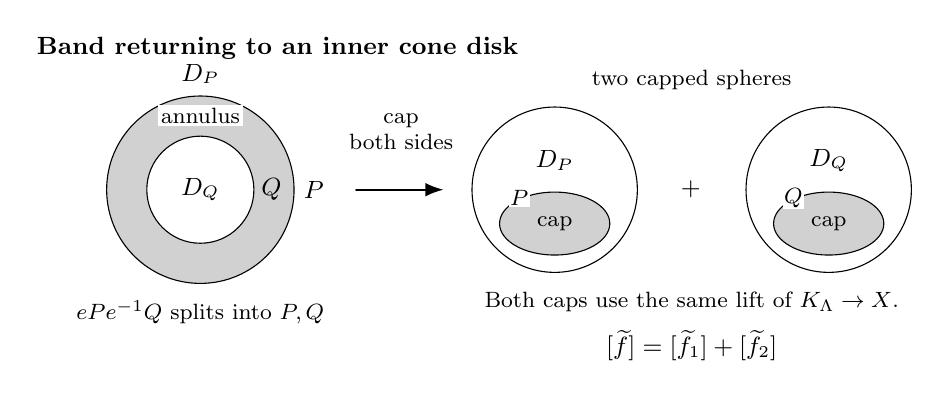
\begin{tikzpicture}[x=1cm,y=1cm,font=\small,
  line cap=round,line join=round,>=Latex]
  \node[anchor=west,font=\small\bfseries] at (0,-2.82)
    {Band returning to an inner cone disk};
  \fill[black!18,even odd rule]
    (2.20,-4.62) circle (1.19cm)
    (2.20,-4.62) circle (0.68cm);
  \draw (2.20,-4.62) circle (1.19cm);
  \draw (2.20,-4.62) circle (0.68cm);
  \node at (2.20,-4.62) {$D_Q$};
  \node at (2.20,-3.15) {$D_P$};
  \node[font=\footnotesize,fill=white,inner sep=1pt]
    at (2.20,-3.68) {annulus};
  \node[anchor=west] at (3.39,-4.62) {$P$};
  \node[anchor=west] at (2.85,-4.62) {$Q$};
  \node[font=\footnotesize,align=center] at (2.20,-6.18)
    {$ePe^{-1}Q$ splits into $P,Q$};

  \draw[->,line width=0.8pt] (4.18,-4.62) -- (5.29,-4.62);
  \node[font=\footnotesize,align=center] at (4.75,-3.88)
    {cap\\both sides};

  \draw (6.70,-4.62) circle (1.05cm);
  \draw (10.18,-4.62) circle (1.05cm);
  \draw[fill=black!18] (6.70,-5.05) ellipse (0.70cm and 0.40cm);
  \draw[fill=black!18] (10.18,-5.05) ellipse (0.70cm and 0.40cm);
  \node at (6.70,-4.25) {$D_P$};
  \node at (10.18,-4.25) {$D_Q$};
  \node[font=\footnotesize] at (6.70,-5.05) {cap};
  \node[font=\footnotesize] at (10.18,-5.05) {cap};
  \node[font=\footnotesize,fill=white,inner sep=0.5pt]
    at (6.25,-4.73) {$P$};
  \node[font=\footnotesize,fill=white,inner sep=0.5pt]
    at (9.73,-4.73) {$Q$};
  \node at (8.43,-4.62) {$+$};
  \node[font=\footnotesize] at (8.44,-3.23)
    {two capped spheres};
  \node[font=\footnotesize] at (8.44,-6.05)
    {Both caps use the same lift of $K_\Lambda\to X$.};
  \node at (8.44,-6.60)
    {$[\widetilde f]=[\widetilde f_1]+[\widetilde f_2]$};
\end{tikzpicture}
\caption{An inner cone disk and its returning band form an annulus,
shown schematically in the domain sphere.  Here $D_P,D_Q$ are its
complementary disks, with boundary paths $P,Q$.  Capping both through
the same abstract cone produces two spheres.  For the original sphere
map $f$, the symbols $[\widetilde f]$ and $[\widetilde f_i]$ denote the
second homology classes of its lift and of the two capped spheres in
the universal cover.  Using for both caps the same lift of
$K_\Lambda\to X$ as for the original annulus gives the displayed
identity.  If $f$ is essential, at least one
capped sphere remains essential.  Shading denotes the annulus and
caps in the domain, without asserting that their images embed in $X$.}
\label{fig:inner-surgery}
\end{figure}


Each case contradicts minimality.  The chosen pairing therefore uses
distinct underlying graph edges.  All the other requirements of
Definition~\ref{def:reduced-arrangement} have already been verified:
the ordinary boundaries are positive and cyclically immersed, there
is at least one such boundary, and the only possible exceptional
boundary is a positive immersed path starting at a designated root.
Thus either failure would give a reduced spherical arrangement.  Its
assumed absence proves both $\pi_2(X)=0$ and root protection.

\subsection{The finite aspherical complex and torsion}

For completeness, we finish the two standard consequences needed in
Proposition~\ref{prop:cone-criterion}.  The universal cover
$\widetilde X$ is simply connected, and the vanishing of $\pi_2(X)$
gives $H_2(\widetilde X;\mathbb Z)=0$ by Hurewicz.  Its higher cellular
homology groups vanish because its dimension is at most two.  Thus it
is simply connected and acyclic.  If it had a nonzero homotopy group,
the first such group would, by Hurewicz, give a nonzero homology group.
All homotopy groups therefore vanish, and Whitehead's theorem makes
$\widetilde X$ contractible.  Hence $X$ is aspherical.  Its finite
two-dimensional CW structure gives a finite presentation for $G$.

The cellular chains of this contractible universal cover give a free
resolution over $\mathbb ZG$,
\[
 0\longrightarrow C_2(\widetilde X)
 \longrightarrow C_1(\widetilde X)
 \longrightarrow C_0(\widetilde X)
 \longrightarrow\mathbb Z\longrightarrow0.
\]
If $G$ had a nonidentity element of finite order, a power of that
element would generate a cyclic subgroup $C_\ell$ of prime order
$\ell$.  Restricting this resolution to $\mathbb ZC_\ell$ still gives
a free resolution of length at most two: $\mathbb ZG$ is a free left
$\mathbb ZC_\ell$-module, with basis given by representatives for the
cosets $C_\ell g$ in $G$.  It would follow that
$H^k(C_\ell;\mathbb F_\ell)=0$ for every $k>2$.

To see the contradiction directly, write $u$ for a generator of
$C_\ell$ and $N=1+u+\cdots+u^{\ell-1}$.  The periodic free resolution
\[
 \cdots\xrightarrow{\,N\,}\mathbb ZC_\ell
 \xrightarrow{\,u-1\,}\mathbb ZC_\ell
 \xrightarrow{\,N\,}\mathbb ZC_\ell
 \xrightarrow{\,u-1\,}\mathbb ZC_\ell
 \longrightarrow\mathbb Z\longrightarrow0
\]
is exact: the augmentation ideal is the image of multiplication by
$u-1$, the kernel of that multiplication is $\mathbb ZN$, and the
kernel of multiplication by $N$ is the
augmentation ideal.  Applying
$\operatorname{Hom}_{\mathbb ZC_\ell}(-,\mathbb F_\ell)$ with trivial
coefficients makes every differential zero, since $u-1$ acts as zero
and $N$ acts as $\ell=0$.  Therefore
$H^k(C_\ell;\mathbb F_\ell)\cong\mathbb F_\ell$ for all $k\ge0$,
the standard cohomological obstruction to torsion in a group of finite
cohomological dimension \cite[Chapter VIII]{Brown1982}.  This
contradiction proves that $G$ is torsion-free and completes the proof
of Proposition~\ref{prop:cone-criterion}.

\section{Completion of the construction}\label{sec:assembly}

We now choose one finite pair of graphs and apply the deterministic results.
\begin{proof}[Proof of Theorem~\ref{thm:main}]
Use the prescribed types of Section~\ref{sec:random} and let
$m\equiv1\pmod4$ tend to infinity. The probability space conditioned on girth
at least $L=\lfloor c_0\log(vm)\rfloor$ is nonempty for sufficiently large
$m$. By Theorem~\ref{thm:no-arrangements}, with probability tending to one
it contains no reduced spherical arrangement. Choose such an outcome with
$L\ge3$, so that both labeled graphs have no loops or parallel edges.

Attach the cones to the rose as in Section~\ref{sec:algebra}, obtaining the
finite two-dimensional complex $X$, and put $G=\pi_1(X)$. By
Proposition~\ref{prop:cone-criterion}, the universal cover of $X$ is
contractible, $G$ is torsion-free, and the labels of paths from either root to
a different vertex of its component are nontrivial in $G$. Finiteness of $X$
gives a finite presentation of $G$.

The intersection parities proved in Proposition~\ref{prop:types} now satisfy
the hypotheses of Proposition~\ref{prop:parity}. That proposition supplies
$a,b,c\in\Ftwo[G]$ with $ab=1$, $ac=0$, and $c\ne0$. Associativity excludes
$ba=1$, as asserted.
\end{proof}

The argument selects a finite matching outcome rather than listing its edges.
Once selected, its cones give a finite presentation, and the sums in
Proposition~\ref{prop:parity} give finite scalar witnesses.


\begingroup
\raggedright
\bibliographystyle{alpha}
\bibliography{references}
\endgroup
\end{document}
